\documentclass[pdflatex, sn-nature]{sn-jnl}\usepackage[]{graphicx}\usepackage[]{xcolor}
% maxwidth is the original width if it is less than linewidth
% otherwise use linewidth (to make sure the graphics do not exceed the margin)
\makeatletter
\def\maxwidth{ %
  \ifdim\Gin@nat@width>\linewidth
    \linewidth
  \else
    \Gin@nat@width
  \fi
}
\makeatother

\definecolor{fgcolor}{rgb}{0.345, 0.345, 0.345}
\newcommand{\hlnum}[1]{\textcolor[rgb]{0.686,0.059,0.569}{#1}}%
\newcommand{\hlstr}[1]{\textcolor[rgb]{0.192,0.494,0.8}{#1}}%
\newcommand{\hlcom}[1]{\textcolor[rgb]{0.678,0.584,0.686}{\textit{#1}}}%
\newcommand{\hlopt}[1]{\textcolor[rgb]{0,0,0}{#1}}%
\newcommand{\hlstd}[1]{\textcolor[rgb]{0.345,0.345,0.345}{#1}}%
\newcommand{\hlkwa}[1]{\textcolor[rgb]{0.161,0.373,0.58}{\textbf{#1}}}%
\newcommand{\hlkwb}[1]{\textcolor[rgb]{0.69,0.353,0.396}{#1}}%
\newcommand{\hlkwc}[1]{\textcolor[rgb]{0.333,0.667,0.333}{#1}}%
\newcommand{\hlkwd}[1]{\textcolor[rgb]{0.737,0.353,0.396}{\textbf{#1}}}%
\let\hlipl\hlkwb

\usepackage{framed}
\makeatletter
\newenvironment{kframe}{%
 \def\at@end@of@kframe{}%
 \ifinner\ifhmode%
  \def\at@end@of@kframe{\end{minipage}}%
  \begin{minipage}{\columnwidth}%
 \fi\fi%
 \def\FrameCommand##1{\hskip\@totalleftmargin \hskip-\fboxsep
 \colorbox{shadecolor}{##1}\hskip-\fboxsep
     % There is no \\@totalrightmargin, so:
     \hskip-\linewidth \hskip-\@totalleftmargin \hskip\columnwidth}%
 \MakeFramed {\advance\hsize-\width
   \@totalleftmargin\z@ \linewidth\hsize
   \@setminipage}}%
 {\par\unskip\endMakeFramed%
 \at@end@of@kframe}
\makeatother

\definecolor{shadecolor}{rgb}{.97, .97, .97}
\definecolor{messagecolor}{rgb}{0, 0, 0}
\definecolor{warningcolor}{rgb}{1, 0, 1}
\definecolor{errorcolor}{rgb}{1, 0, 0}
\newenvironment{knitrout}{}{} % an empty environment to be redefined in TeX

\usepackage{alltt}

\usepackage{fullpage}
\usepackage{amsmath}
\usepackage{url}
\usepackage{booktabs}
\usepackage{placeins}
\usepackage{xr}

\usepackage[font=small]{caption}

%\urlstyle{same}
\newcommand{\degr}{$^{\circ{}}$C}

\renewcommand{\figurename}{Supplementary Figure}
\renewcommand\refname{Supplementary References}

\externaldocument[ED-]{../extended_data/ext_data}
\IfFileExists{upquote.sty}{\usepackage{upquote}}{}
\begin{document}

\title{Shifting hail hazard under global warming and effects on crop hail exposure: supplementary information}

\author*[1,2,3,4]{\fnm{Timothy H.} \sur{Raupach}}\email{timothy.h.raupach@gmail.com}
\author[5,6]{\fnm{Raphael} \sur{Portmann}}
\author[7]{\fnm{Christian} \sur{Siderius}}
\author[2,3,4]{\fnm{Steven C.} \sur{Sherwood}}

\affil[1]{\orgdiv{Institute for Climate Risk and Response}, \orgname{UNSW Sydney}, \orgaddress{\street{Mathews Building Level 4}, \city{The University of New South Wales, Sydney}, \postcode{2051}, \state{NSW}, \country{Australia}}}
\affil[2]{\orgdiv{Climate Change Research Centre}, \orgname{UNSW Sydney}, \orgaddress{\country{Australia}}}
\affil[3]{\orgdiv{ARC Centre of Excellence for Climate Extremes}, \orgname{UNSW Sydney}, \orgaddress{\country{Australia}}}
\affil[4]{\orgdiv{ARC Centre of Excellence for 21st Century Weather}, \orgname{UNSW Sydney}, \orgaddress{\country{Australia}}}
\affil[5]{\orgdiv{Agroscope}, \orgname{Swiss Federal Office for Agriculture}, \orgaddress{\city{Zurich}, \country{Switzerland (prev. address)}}}
\affil[6]{\orgname{Planval}, \orgaddress{\city{Bern}, \country{Switzerland}}}
\affil[7]{\orgname{Uncharted Waters}, \orgaddress{\city{Sydney}, \country{Australia}}}

\maketitle



\newpage
\section*{Contents}

This supplementary material contains:

\begin{itemize}
\item Section \ref{sec:proxy_validation}: A validation of proxy climatologies via comparison with published climatologies.
\item Section \ref{sec:supp_figures}: Supplementary tables and figures: Supplementary Table \ref{tab:model_details} and Supplementary Figures \ref{fig:anoms_India_2015}--\ref{fig:epochs}.
\item Section \ref{sec:proxy-formulas}: A detailed description of the proxies used in this study.
\end{itemize}

\section{Validation of proxy climatologies}
\label{sec:proxy_validation}

We used normalised proxies because individual model/proxy combinations produced
varying numbers of hail-prone days (Extended Data Figure
\ref{ED-fig:historical_annual_means}). The three proxies we used were trained
locally in Australia (Raupach), Italy (Eccel), and the USA (SHIP), which raises
the question of whether they can reasonably be applied globally. In this section
we compare, in detail, the proxy ensemble output we use in this work to
published climatologies by world region. For global climatologies we compared to
the proxy-based climatology of Prein \& Holland, 2018 (\cite{Prein_WCE_2018},
hereafter PH18) and the satellite-based climatology of Bang \& Cecil, 2019
(\cite{Bang_JAMC_2019}, hereafter BC19) while noting that both these global
climatologies are for severe or large hail, and the proxies we use in this study
are chosen to detect \textit{any} hail-prone conditions (with the low threshold
we used for POH). We thus expect some differences with these previous global
climatologies. There are no ``perfect'' hail observations because hail is small
in scale and relatively rare, radars and observations networks have limited
spatial coverage, reports contain non-meteorological biases, and there are
significant uncertainties in linking large-scale environments (using proxies) or
observations aloft by satellite or radar to surface hail occurrence
\citep{Raupach_NREE_2021}. The climatological studies we compared to included
all available data sources including proxies, radar, satellite, and
observations/reports. We used as many studies as possible for each region, to
incorporate local knowledge, observations, and model training into our global
proxy validation. Differences in geographical supports, observation techniques,
reporting standards, and the mixture of direct and indirect methods to estimate
hail occurrence in the literature mean that it is not feasible to compare
absolute numbers of hail occurrences or hail-prone days between climatologies.
Instead, we focused on whether there is agreement in relative hail activity by
region. Regional commentary and comparisons are shown in the following
subsections, in which we use the region and subregions definitions of the United
Nations geoscheme \citep{UN_geoscheme}.

\subsection{Areas referred to in the main text}
\label{sec:regions}

In the main paper, we use the following shorthand definitions to refer to the
following regions of the United Nations geoscheme \citep{UN_geoscheme}. ``Asia''
refers to Southern, Eastern, Northern, and northern South-eastern Asia as shown
in Figure \ref{fig:proxy_climatology_asia}; ``Oceania'' refers to Oceania and
southern South-eastern Asia as shown in Figure
\ref{fig:proxy_climatology_oceania}; ``North America'' refers to Northern
America, Central America, and the Caribbean, as shown in Figure
\ref{fig:proxy_climatology_north_america}; ``South America'' refers to South
America as shown in Figure \ref{fig:proxy_climatology_south_america}; ``Europe''
refers to Europe, Northern Africa, Western Asia, and Iran as shown in Figure
\ref{fig:proxy_climatology_europe}; and ``Africa'' refers to Africa as shown in
Figure \ref{fig:proxy_climatology_africa}.

\subsection{Southern, Eastern, Northern, and northern South-eastern Asia}

\begin{figure}[h]
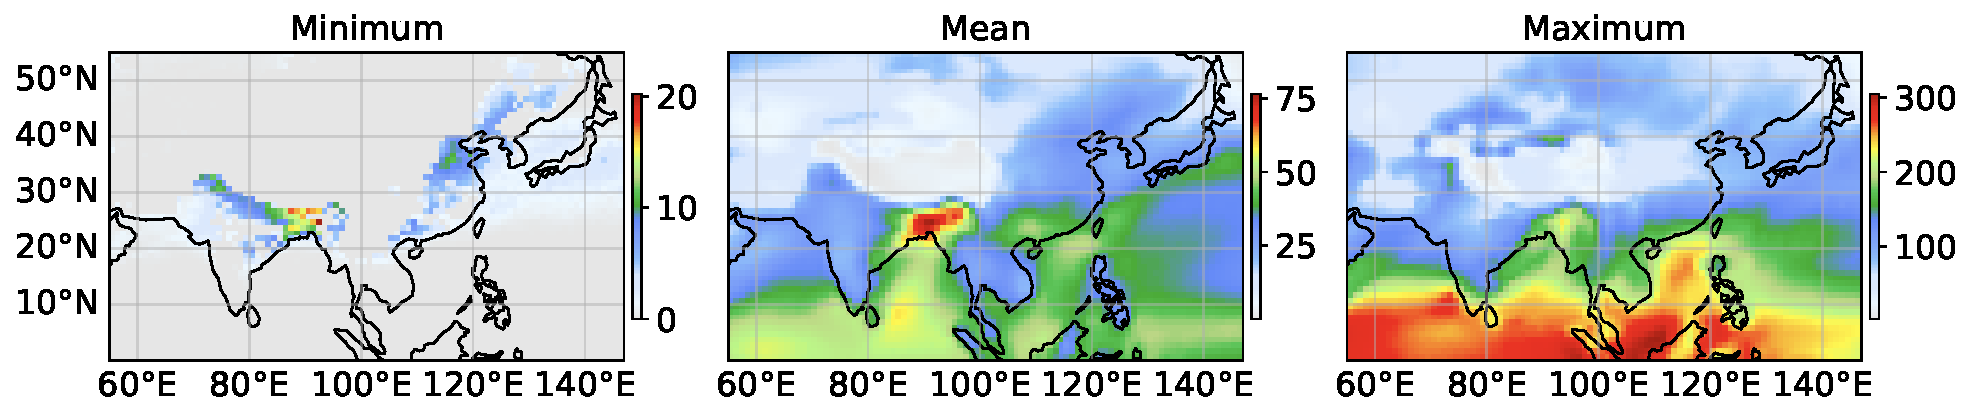
\includegraphics[width=\textwidth]{../../results/supplementary/proxy_climatology_asia}
\caption{Mean and standard deviation of normalised annual hail-prone days across
the model-proxy ensemble for the historical period, including CMIP6 models and
ERA5 reanalysis, for Southern, Eastern, Northern, and northern South-eastern
Asia. Solid black lines show coastlines and political borders; dotted black
lines show provincial boundaries for some countries.}
\label{fig:proxy_climatology_asia}
\end{figure}

In Asia, the proxy ensemble (Figure \ref{fig:proxy_climatology_asia}) highlights
the southern flank of the Himalaya and particularly its southeastern end as the
most hail-prone region, with another hotspot in southern China, and low hail
probability across the Tibetan plateau. This pattern matches a satellite severe
hail climatology \citep{Bang_JAMC_2019} and is similar to the severe hail
climatology of PH18, except that study shows another hotspot in the northeast of
Pakistan which is not matched by the proxy ensemble or by BC19. Regional studies
confirm that the northwestern Himalaya \citep{Bhat_NH_2024}, North, Northeast,
and East India \citep{Rao_NH_2025}, Northern Thailand \citep{Mahavik_NH_2025},
and Southwestern China \citep{Li_JAMC_2018} are hail hotspots. Hail is also
reported across some parts of Central India \citep{Rao_NH_2025,
Ravindren_NH_2025} where satellite and proxy products show only moderate hail
probability. Hail in Western Siberia is infrequent but does occur in the regions
highlighted by the proxy ensemble \citep{Gorbatenko_RMH_2020}. Station-based
climatologies in China show high hail occurrence over the Tibetan Plateau
\citep{Zhang_JAMC_2008, Li_JAMC_2018}, disagreeing with both proxy and satellite
studies. In summary, the proxy ensemble agrees well with published climatologies
for Southern, Eastern, Northern, and northern South-eastern Asia, except for the
Tibetan Plateau where the ensemble agrees with satellite and proxy climatologies
but disagrees with station data.

\FloatBarrier

\subsection{Oceania and southern South-eastern Asia}
\label{sec:oceania}

\begin{figure}[h]
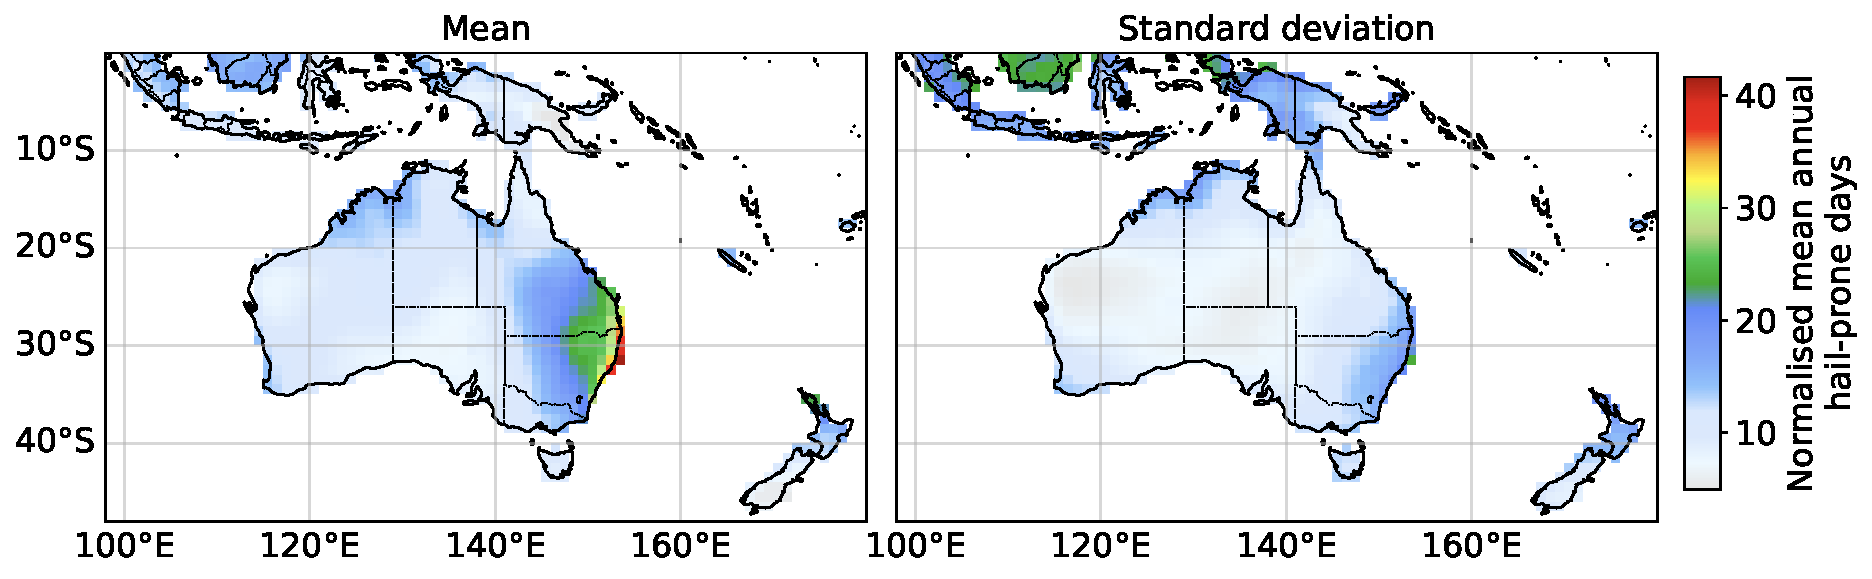
\includegraphics[width=\textwidth]{../../results/supplementary/proxy_climatology_oceania}
\caption{As for Figure \ref{fig:proxy_climatology_asia} but for Oceania.}
\label{fig:proxy_climatology_oceania}
\end{figure}

In Oceania, the proxy ensemble (Figure \ref{fig:proxy_climatology_oceania})
shows high hail probability on the mid-eastern coast of Australia with higher
hail probability in the country's northwest and low probability in the arid
centre, some hail activity in New Zealand's North Island but lower probabilities
in the South Island, and moderate hail activity in Indonesia.
PH18 and BC19 both show regions of higher
severe hail probability on the mid-eastern and northern coasts of Australia and
moderate probabilities in Australia's northwest. PH18's results
suggest the possibility of hail activity in Australia's southwest and western
interior, where the ensemble generally shows low probability (although some
ensemble members show hail activity in the far southwest). BC19
shows low but non-zero severe hail probability across the western Maritime
Continent, agreeing with the ensemble but disagreeing with
PH18. The ensemble and PH18 agree on the North
Island of New Zealand showing higher hail probability than the South Island.
Regional studies confirm the hail occurrence peak on Australia's east coast
\citep{Raupach_npjCAS_2023, Brook_MWR_2024} and the possibility of a hail
hotspot in the southwest \citep{Raupach_npjCAS_2023, Brook_MWR_2024,
Bedka_JAMC_2018}, while hail in Australia's tropics is subject to uncertainty
\citep{Raupach_MWR_2023, Bedka_JAMC_2018, Prein_WCE_2018}. In New Zealand,
hailstorm occurrence is recorded as increasing towards the west and south
\citep{Steiner_NZJGG_1989}, but recent data are scarce. In Indonesia there are
few studies but damaging hailstorms do occur \citep{Sari_JGRA_2025}. Overall,
the proxy ensemble agrees well with the locations of known hail hotspots in
Oceania and southern South-eastern Asia.

\FloatBarrier

\subsection{Northern America, Central America, and the Caribbean}

\begin{figure}[h]
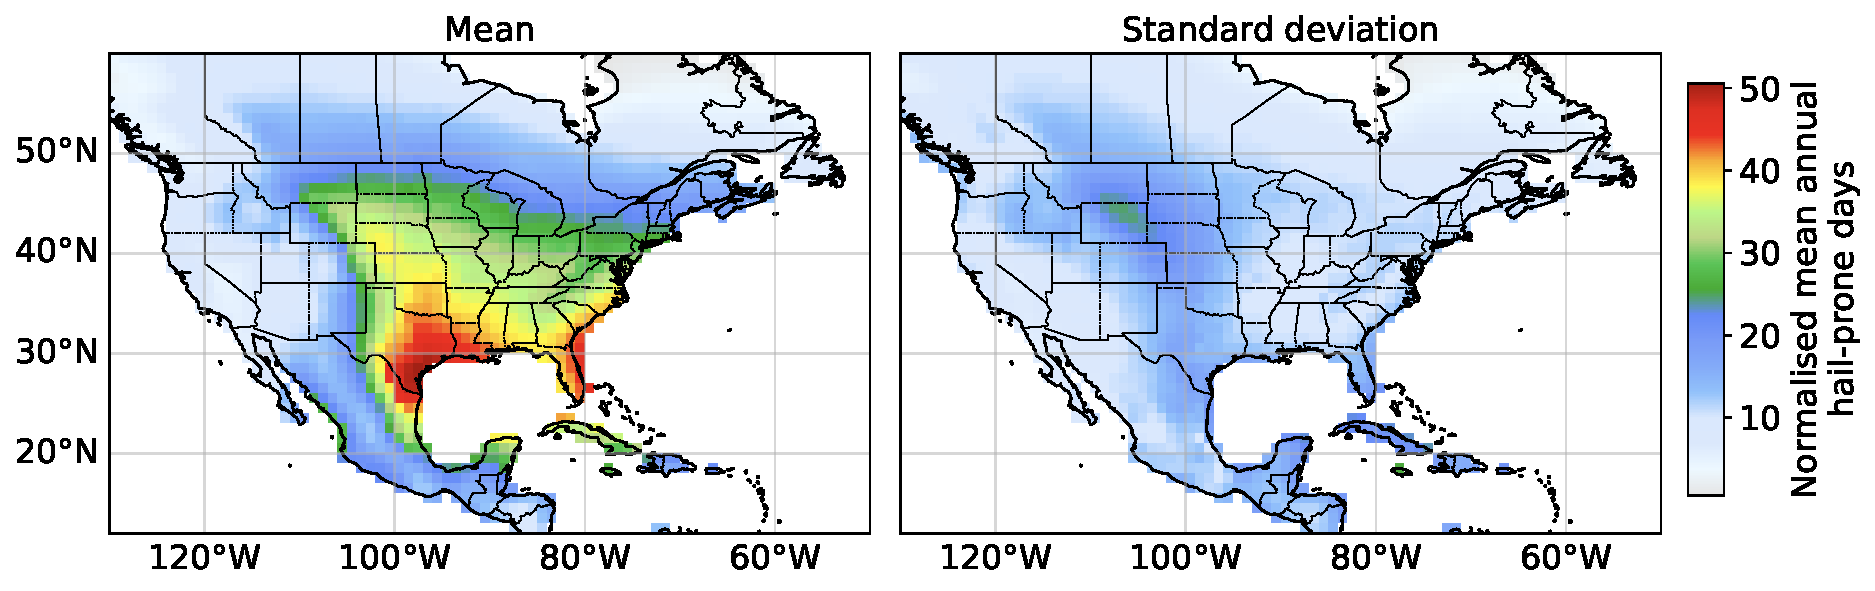
\includegraphics[width=\textwidth]{../../results/supplementary/proxy_climatology_north_america}
\caption{As for Figure \ref{fig:proxy_climatology_asia} but for Northern
America, Central America, and the Caribbean.}
\label{fig:proxy_climatology_north_america}
\end{figure}

The proxy ensemble (Figure \ref{fig:proxy_climatology_north_america}) shows
hail-prone areas in Northern America as lying to the east of the Rocky Mountains
with the highest occurrence of hail-prone conditions in the southeast United
States of America (USA), along the Gulf of Mexico and eastern Florida. In
addition, the ensemble shows hail-prone conditions extending north into Canada
with the furthest extension in Alberta, and extending south into Central
America, with a thin region of increased probability along the west coast of
Mexico. The severe hail climatology of PH18 highlights a similar overall region
of risk and also shows increased hail risk in Mexico's west, albeit a little
further inland. However, PH18 has the highest probability area in the USA
extending further north across the Great Plains than the proxy ensemble.
Satellite-based detections also highlight similar regions as the proxy ensemble,
but put the greatest occurrence across the US Great Plains and Cuba
\citep{Bang_JAMC_2019}. Extended Data Figure
\ref{ED-fig:historical_annual_means} shows that the latitude of the peak in
hail-prone conditions changes by proxy and model in our results. Regional
climatologies confirm that the most hail-prone areas of the United States is the
Great Plains east of the Rocky Mountains, and that there is a strong east-west
divide with little hail occurrence to the west of the Rocky Mountains
\citep{Cintineo_WF_2012, Allen_EJSSM_2015, Allen_JAMES_2015, Murillo_MWR_2021}.
A radar-based climatology shows outlier hotspots in Florida and the eastern
sides of Georgia and South Carolina \citep{Cintineo_WF_2012}, and hail reports
exist in most areas east of the Rocky Mountains \citep{Allen_JAMES_2015}. In
Canada, the highest hail probability region is across southern Manitoba and
Saskatchewan and extending northwards into Alberta \citep{Brunet_JAMC_2024}
which agrees well with the ensemble climatology. In Mexico, hailstorms occur
over the high-elevation parts of the south and northwest
\citep{Leon-Cruz_IJC_2023}, aligning with the ensemble's increased hail
probability along the northwest Mexico coast. In summary, while some proxy
ensemble members underestimate the hail probability in the northern Great Plains
of the United States and others overestimate hail probability along the Gulf
Coast, the ensemble reasonably captures the overall spatial distribution of
hail-prone areas in Northern America, Central America, and the Caribbean.

\FloatBarrier

\subsection{South America}

\begin{figure}[h]
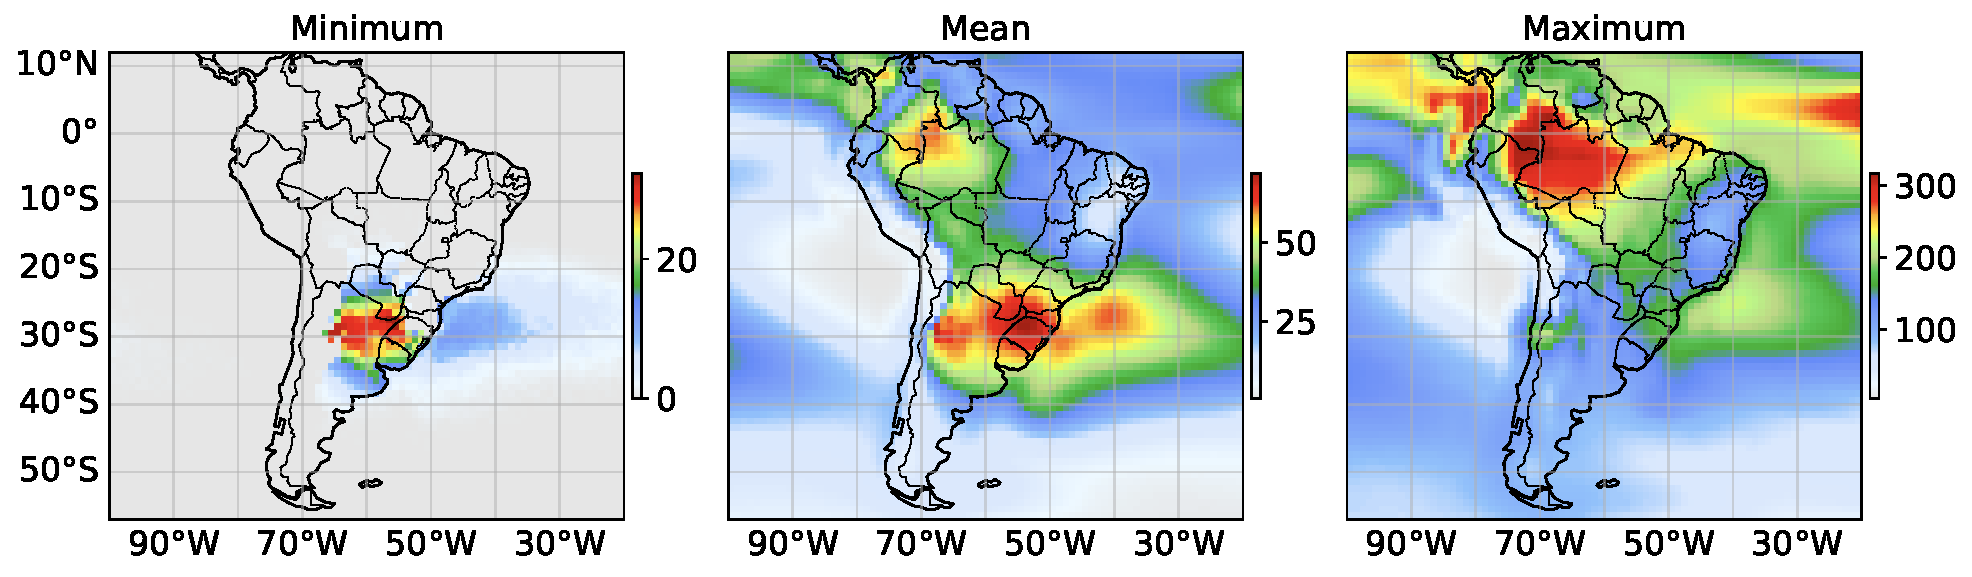
\includegraphics[width=\textwidth]{../../results/supplementary/proxy_climatology_south_america}
\caption{As for Figure \ref{fig:proxy_climatology_asia} but for South America.}
\label{fig:proxy_climatology_south_america}
\end{figure}

In South America, the proxy ensemble (Figure
\ref{fig:proxy_climatology_south_america}) shows regions of higher probability
of hail-prone conditions to the east of the Andes, with hotspots in northern
Argentina, Uruguay, southern Paraguay, southern Brazil, southern Bolivia, the
northwest corner of Colombia, and a region covering southeastern Columbia,
southern Venezuela, and northeastern Peru. PH18 shows agreement
for northwestern Argentina with hail probability extending into Uruguay and
Bolivia, but show less hail activity than the proxy ensemble in the north of
the continent. BC19 further confirms the hotspot in the proxy
ensemble over northern Argentina/Uruguay/Paraguay/southern Brazil as well as the
hotspot in northwest Colombia. Regional studies show that northern Argentina and
the border region between Brazil, Argentina and Paraguay is a hail hotspot
\citep{Beal_AR_2020, Nesbitt_BAMS_2021, Bruick_MWR_2019, Martins_AR_2017,
Mezher_AR_2012}. Southern Brazil is well established as a region that
experiences frequent destructive hailstorms \citep{Martins_AR_2017}. A regional
climatology in Argentina shows hotspots in the mid-northwest and northeast,
which are captured by the proxy ensemble, and an isolated hotspot in the south
which the ensemble does not capture \citep{Mezher_AR_2012}. In the north of
South America, hailstorms are known to occur in the Central Andes of Peru
\citep{Valdivia_AMT_2024}. In Colombia, hail is reported across the whole
country, but the most hail-prone regions are in the western, central and eastern
branches of the Andes (the ensemble highlights the eastern side), and in the
Sierra Nevada de Santa Marta in the country's north, which agrees well with the
ensemble \citep{Pena_Beltran_CG_2020}. There is a notable region of
within-ensemble variability across the Peru/Colombia/Brazil border region. The
proxy ensemble captures well the most hail-prone regions in South America.

\FloatBarrier

\subsection{Europe, Northern Africa, Western Asia, and Iran}
\label{sec:europe}

\begin{figure}[h]
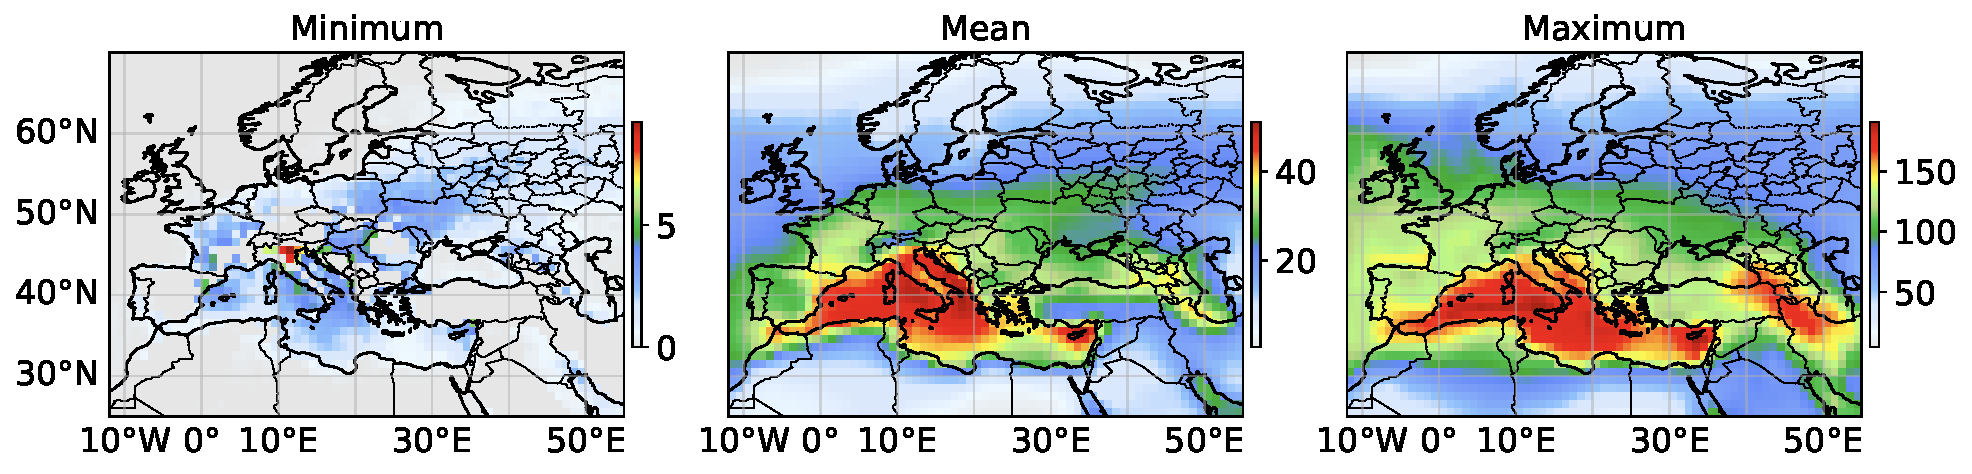
\includegraphics[width=\textwidth]{../../results/supplementary/proxy_climatology_europe}
\caption{As for Figure \ref{fig:proxy_climatology_asia} but for Europe, Northern
Africa, and Western Asia.}
\label{fig:proxy_climatology_europe}
\end{figure}

In Europe, Northern Africa, Western Asia, and northern Iran, the proxy ensemble
(Figure \ref{fig:proxy_climatology_europe}) shows hail hotspots in Italy
(especially its north), Croatia, the foothills of the Alps, eastern Spain, and a
swath that runs from southeast to northwest France and into southern Germany.
The high Alps are a local minimum in hail-prone conditions. Hail-prone regions
extend eastwards across Hungary, Romania, and across the Black Sea to Georgia,
Armenia, Azerbaijan, and northern Iran. The ensemble shows the Mediterranean
coasts as particularly hail prone, and the northern edges of the African
continent show hail-prone conditions, particularly in Morocco.
PH18 agrees well, showing similar peaks in northern Italy and
the Pyrenees, the diagonal band across France, the minimum over the high Alps,
the hotspot in eastern Spain, hail-prone conditions in Northern Africa, and the
eastwards extension of hail-prone conditions to northern Iran.
BC19 shows the highest number of hail detections in the
Mediterranean Sea to the southeast of Italy, and generally agrees with the
distribution of hail-prone regions in the ensemble, although the low resolution
of the satellite data somewhat hampers detailed comparison. Regional
climatologies broadly align with the proxy ensemble's distribution of hail-prone
regions. By subregion:

\begin{itemize}
    \item \textbf{Eastern Europe:} The Northern Caucasus has high hail
    occurrence for Eastern Europe \citep{Malkarova_RMH_2011,
    Zharashuev_RMH_2012, Punge_AR_2016}, hail occurs on the Crimean Peninsular
    \citep{Zharashuev_RMH_2012} and in western and southern Russia \citep[][and
    references therein]{Punge_AR_2016}, and large hail has been reported in
    Belarus \citep{Punge_AR_2016}.  In Romania, hail occurs across the country
    \citep{Istrate_GT_2017} with a probable higher concentration in the west
    \citep{Burcea_MWR_2016}; hail frequency increases from the southeast to the
    north and west, and the northwest is a known hotspot \citep{Punge_AR_2016}.
    The Republic of Moldova experiences significant agricultural damage from
    hail \citep{Potapov_RMH_2007}. Hail is common in Bulgaria
    \citep{Simeonov_AR_2009}. In Hungary, Slovakia, and Poland, environmental
    conditions for hail increase in frequency toward the southeast
    \citep{Mohr_GRL_2015}. In Poland there are few hailstorms in the north
    \citep[][and citations therein]{Punge_AR_2016}. The ensemble shows
    relatively uniform hail-prone conditions occurrence for Czechia and
    Slovakia: station data show that Czechia experiences more hail hazard than
    Poland, and more than Slovakia where reports of hail are relatively few
    \citep{Punge_AR_2016}. In Poland, weather stations record hail slightly more
    frequent hail than those in northern Germany, and there is a reported
    minimum in frequency in the southeast \citep{Suwala_QG_2013}, which is not
    shown in the proxy ensemble. Modelling shows more simulated hail in Eastern
    Europe than in Western Europe \citep{Cui_JGRA_2025}. Except for the reported
    minimum in southeast Poland, the ensemble agrees well with published
    climatologies in Eastern Europe.

    \item \textbf{Northern Europe:} Hail is generally uncommon in Northern
    Europe \citep{Punge_AR_2016}. Hail is uncommon in Norway and Denmark
    \citep{Tuovinen_MWR_2009}, but somewhat more frequent in Sweden \citep[][and
    references therein]{Punge_AR_2016}. Finland experiences damaging hail,
    especially in the south and west and rarely in the north
    \citep{Tuovinen_MWR_2009}. In Estonia and Lithuania hail occurs but is not
    common \citep[][and references therein]{Punge_AR_2016}. Hail is uncommon in
    Ireland and the United Kingdom of Great Britain and Northern Ireland, with
    decreasing hail activity from east to west \citep{Mohr_GRL_2015,
    Punge_AR_2016}. These patterns are well captured by the ensemble
    climatology.

    \item \textbf{Southern Europe:} In Portugal, hail is reported mostly in the
    north \citep{Santos_IJC_2019}. In Spain, supercells including hail occur
    particularly in the east along the Mediterranean coast
    \citep{Calvo-Sancho_WCD_2022}, hail is reported most frequently in the east
    and northeast \citep{Saa-Requejo_NHESS_2011}, and conditions are most
    hail-prone along the Mediterranean coast \citep{Mohr_AR_2013}; these regions
    are corroborated by modelling \citep{Cui_JGRA_2025}. Agricultural damages
    from hail are high in the northeast of Spain \citep[][and references
    therein]{Punge_AR_2016}. In Italy, hail occurs across the country but with
    greatest frequency in the north and with regions of lower frequency across
    Central Italy \citep{Baldi_AR_2014, Cui_JGRA_2025}. The pre-alps of Northern
    Italy are among the most hail-prone regions of Europe \citep{Mohr_AR_2013,
    Cui_JGRA_2025, Punge_AR_2016}. In Bosnia and Herzegovina, hailstorms damage
    crops in the north \citep{Dejanovic_2019}. In Serbia, hail occurs most
    frequently in the southwest \citep{Curic_IJC_2016}. Hail is common in
    Slovenia \citep{Punge_AR_2016}, Macedonia \citep{Dimitrievski_JWM_1983}, and
    northern Greece \citep{Sioutas_AR_2009} but less common in southern Greece
    \citep{Punge_AR_2016}. Croatia is hail-prone with high frequency toward the
    coast \citep{Blaskovic_AR_2023, Jelic_JGRA_2020, Mohr_GRL_2015}. Overall,
    the ensemble outputs align with regional climatologies for Southern Europe.

    \item \textbf{Western Europe:} In France, there is a diagonal band of higher
    hail frequency extending from the southwest to northeast, with lower hail
    frequencies in the northwest and southeast
    \citep{Vinet_AR_2001,Fluck_NHESS_2021,Mohr_AR_2013,Cui_JGRA_2025}. The
    southwest near the Pyrenees is particularly hail prone
    \citep{Vinet_AR_2001,Berthet_AR_2011, Berthet_AR_2013} while the Massif
    Central in the centre-east shows high hail activity in radar data
    \citep{Fluck_NHESS_2021} but low activity in an environment-based analysis
    \citep{Mohr_AR_2013}. The ensemble reproduces this overall structure for
    France, although the ensemble's SW-NE band extends slightly further to the
    northwest than those shown in Vinet 2001 \cite{Vinet_AR_2001} and Fluck et
    al., 2021 \cite{Fluck_NHESS_2021}. The frequency of hail-prone conditions
    decreases towards the Atlantic coasts of France, Belgium, and The
    Netherlands \citep{Mohr_GRL_2015, Punge_AR_2016}, and Belgium has lower hail
    frequency than neighbouring regions of France and Germany
    \citep{Lukach_MA_2017, Fluck_NHESS_2021}. In Germany, hail hazard is higher
    in the southern half of the country
    \citep{Mohr_GRL_2015, Fluck_NHESS_2021, Suwala_QG_2013, Cui_JGRA_2025, Punge_AR_2016}
    with hotspots in the Black Forest region \citep{Fluck_NHESS_2021,
    Suwala_QG_2013, Nisi_QJRMS_2016} and a minimum in the northern lowlands
    \citep{Suwala_QG_2013}. In radar data from Switzerland, the pre-alps to the
    north and south of the main Alpine chain, the Black Forest region in
    southwest Germany, and the Jura mountains on the border between Switzerland
    and France, are hail-prone \citep{Nisi_QJRMS_2016}. The high Alps show
    little hail activity \citep{Mohr_GRL_2015, Nisi_QJRMS_2016,
    Kahraman_MWR_2016, Punge_AR_2016}, as reproduced by the ensemble. Hail-prone
    regions in Austria are to the east, out of the main Alpine chain
    \citep{Svabki_ECSS_2013,Punge_AR_2016}. The proxy ensemble aligns closely
    with published regional climatologies for Western Europe.

    \item \textbf{Northern Africa:} There is little detailed climatological
    information for hail in Northern Africa. Hail occurrence is shown across
    Northern Africa in the Mediterranean hail climatology of Laviola et al.,
    2022 \cite{Laviola_RS_2022}, with highest occurrence in Autumn in the region
    around Libya, which aligns with the ensemble climatology.
    
    \item \textbf{Western Asia and Iran:} T\"{u}rkiye is affected by hail, with
    reports concentrated on its Mediterranean coasts in the cold season and
    across the country in summer, with a maximum in hail days in the northeast
    \citep{Kahraman_MWR_2016}. In Armenia, hail is a significant hazard to
    agriculture \citep{Arazyan_EDR_2020}, with higher hail occurrence in the
    north \citep{Harutyunyan_2017}. Georgia is known to be hail prone,
    especially in the east \citep{Varazanashvili_NH_2012} but with hail
    occurring across the territory \citep{Tatishvili_JGGS_2017}. Hail is common
    in Cyprus \citep{Michaelides_NHESS_2008, Nicolaides_AG_2009}. In Iran, hail
    occurs with more prominence in the mountainous regions
    \citep{Salahi_JESS_2018}, and crop losses are recorded in the northwest
    \citep{MirMousavi_JPHGR_2022}. These patterns across Western Asia and Iran
    are well captured by the proxy ensemble.
\end{itemize}

\FloatBarrier

\subsection{Africa}

\begin{figure}[h]
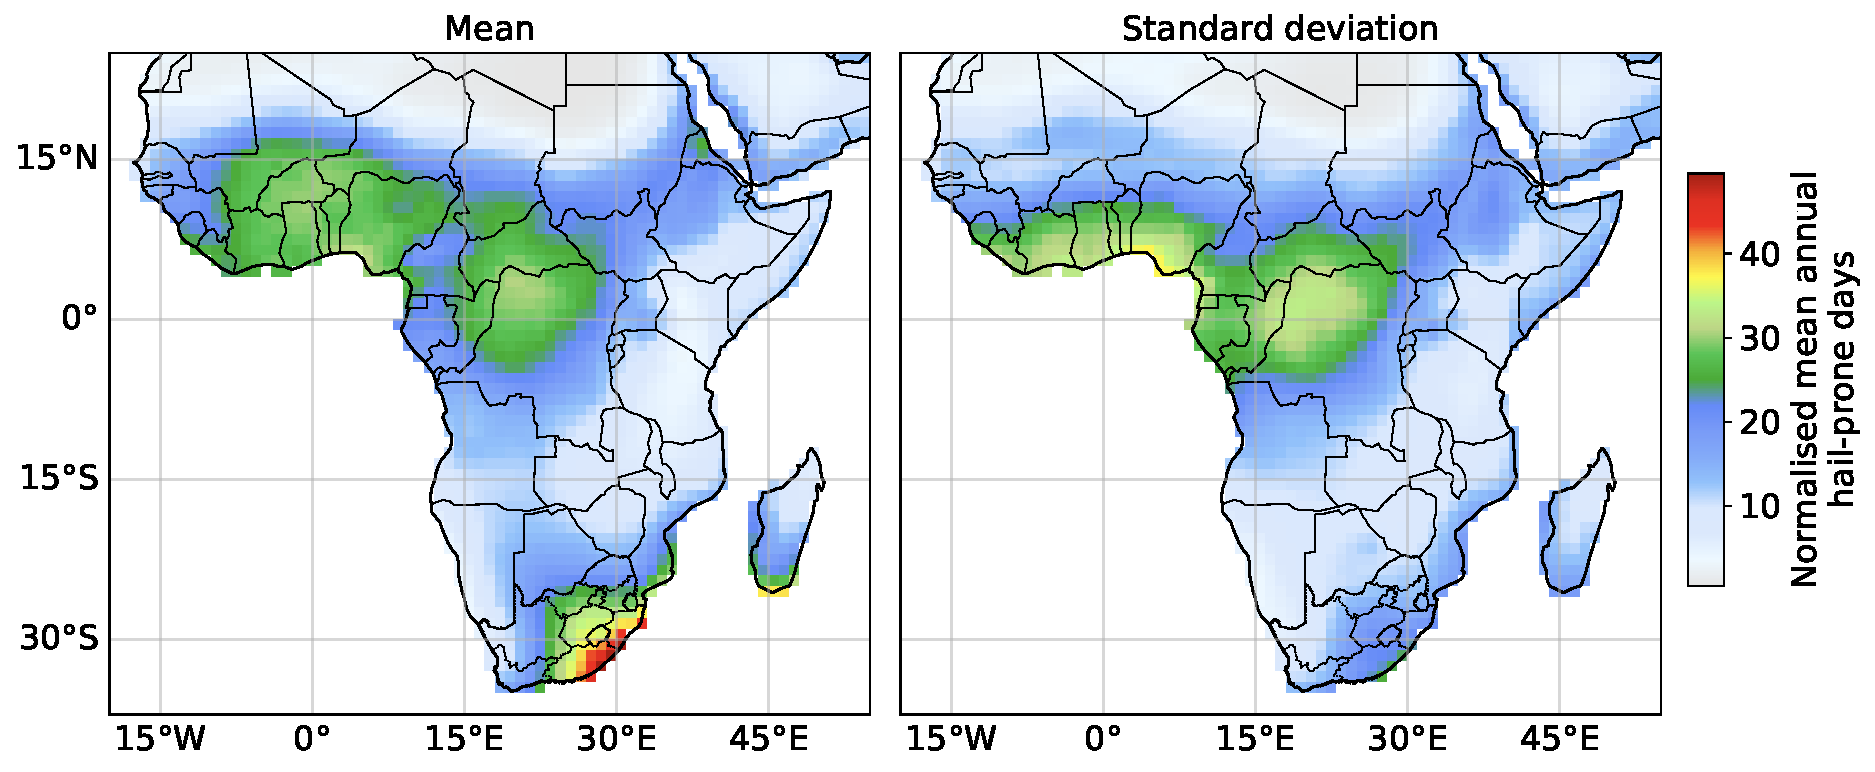
\includegraphics[width=\textwidth]{../../results/supplementary/proxy_climatology_africa}
\caption{As for Figure \ref{fig:proxy_climatology_asia} but for Africa.}
\label{fig:proxy_climatology_africa}
\end{figure}

In Africa, the proxy ensemble (Figure \ref{fig:proxy_climatology_africa}) shows
a band of high hail potential across the sub-Saharan tropics, with hotspots on
the coasts of Nigeria, Benin, and Togo, uniform hail-prone condition occurrence
across Ghana and higher occurrence in the east of C\^ote D'Ivoire, as well as a
hotspot in northwest Democratic Republic of the Congo and the border region with
the Central African Republic and Republic of the Congo. The region extends with
lower hail-prone condition occurrence to the east across South Sudan, southern
Sudan and northern Ethiopia, and to Eritrea. In the south, the obvious hotspot
is in eastern South Africa, where hail-prone conditions spread northwest to the
border with Botswana and north along the east coast into Mozambique. The
southern tip of Madagascar is shown as hail-prone. PH18 and the ensemble broadly
agree on the eastern South Africa and tropical hotspots, though PH18's high
magnitudes are slightly to the north and east of those in the ensemble, and
further inland, and they show hotspots in Angola and in Uganda near Lake
Victoria, both regions in which the ensemble shows reduced hail risk. BC19
broadly agrees with the ensemble, with a large tropical region of high numbers
of hail detections and hotspots in eastern South Africa and Madagascar. Regional
climatologies for southern Africa confirm the eastern South Africa hail hotspot
\citep{Dyson_IJC_2021, Punge_NHESS_2023} with most severe thunderstorm
environments occurring near the coast \citep{Blamey_CD_2017}, although the
reanalysis-based climatology of Dyson et al., 2021 \cite{Dyson_IJC_2021} places
the hail activity maximum slightly further inland. Hail climatology over
tropical Africa remains subject to uncertainty \citep{Bang_JAMC_2019,
Ni_JAMC_2017} with few regional climatologies available, but hail occurs
relatively often in western Kenya \citep{Stephens_AFM_1992, Frisby_JAMC_1967}
and has been reported, mostly rarely, across the rest of the African tropics
\citep{Frisby_JAMC_1967}. Except for missing possible hail activity near Lake
Victoria, the proxy ensemble agrees reasonably well with the limited
climatological information available for Africa.

\FloatBarrier

\newpage
\section{Supplementary tables and figures}
\label{sec:supp_figures}

% latex table generated in R 4.3.3 by xtable 1.8-4 package
% Wed Apr  8 17:36:44 2026
\begin{table}[h]
\centering
\begingroup\footnotesize
\begin{tabular}{llllrrlll}
  \toprule
Model & Institution & Experiment & Ensemble & Start & End & Res & Vert & Orog \\ 
  \midrule
CMCC-CM2-SR5 & CMCC & historical & r1i1p1f1 & 1980 & 1999 & 100 km & 30.0 &  \\ 
  CMCC-CM2-SR5 & CMCC & ssp585 (2C) & r1i1p1f1 & 2037 & 2056 & 100 km & 30.0 &  \\ 
  CMCC-CM2-SR5 & CMCC & ssp585 (3C) & r1i1p1f1 & 2054 & 2073 & 100 km & 30.0 &  \\ 
  CMCC-ESM2 & CMCC & historical & r1i1p1f1 & 1980 & 1999 & 100 km & 30.0 &  \\ 
  CMCC-ESM2 & CMCC & ssp585 (2C) & r1i1p1f1 & 2041 & 2060 & 100 km & 30.0 &  \\ 
  CMCC-ESM2 & CMCC & ssp585 (3C) & r1i1p1f1 & 2056 & 2075 & 100 km & 30.0 &  \\ 
  CNRM-CM6-1 & CNRM-CERFACS & historical & r1i1p1f2 & 1980 & 1999 & 250 km & 91.0 &  \\ 
  CNRM-CM6-1 & CNRM-CERFACS & ssp585 (2C) & r1i1p1f2 & 2042 & 2061 & 250 km & 91.0 & X \\ 
  CNRM-CM6-1 & CNRM-CERFACS & ssp585 (3C) & r1i1p1f2 & 2057 & 2076 & 250 km & 91.0 & X \\ 
  EC-Earth3 & EC-Earth-Consortium & historical & r1i1p1f1 & 1980 & 1999 & 100 km & 91.0 &  \\ 
  EC-Earth3 & EC-Earth-Consortium & ssp585 (2C) & r1i1p1f1 & 2031 & 2050 & 100 km & 91.0 &  \\ 
  EC-Earth3 & EC-Earth-Consortium & ssp585 (3C) & r1i1p1f1 & 2052 & 2071 & 100 km & 91.0 &  \\ 
  GISS-E2-1-G & NASA-GISS & historical & r1i1p1f2 & 1980 & 1999 & 250 km & 40.0 & X \\ 
  GISS-E2-1-G & NASA-GISS & ssp585 (2C) & r1i1p1f2 & 2028 & 2047 & 250 km & 40.0 & X \\ 
  GISS-E2-1-G & NASA-GISS & ssp585 (3C) & r1i1p1f2 & 2055 & 2074 & 250 km & 40.0 & X \\ 
  MIROC6 & MIROC & historical & r1i1p1f1 & 1980 & 1999 & 250 km & 81.0 &  \\ 
  MIROC6 & MIROC & ssp585 (2C) & r1i1p1f1 & 2051 & 2070 & 250 km & 81.0 &  \\ 
  MIROC6 & MIROC & ssp585 (3C) & r1i1p1f1 & 2072 & 2091 & 250 km & 81.0 &  \\ 
  MPI-ESM1-2-HR & MPI-M & historical & r1i1p1f1 & 1980 & 1999 & 100 km & 95.0 &  \\ 
  MPI-ESM1-2-HR & DKRZ & ssp585 (2C) & r1i1p1f1 & 2053 & 2072 & 100 km & 95.0 &  \\ 
  MPI-ESM1-2-HR & DKRZ & ssp585 (3C) & r1i1p1f1 & 2075 & 2094 & 100 km & 95.0 &  \\ 
  MRI-ESM2-0 & MRI & historical & r1i1p1f1 & 1980 & 1999 & 100 km & 80.0 &  \\ 
  MRI-ESM2-0 & MRI & ssp585 (2C) & r1i1p1f1 & 2038 & 2057 & 100 km & 80.0 &  \\ 
  MRI-ESM2-0 & MRI & ssp585 (3C) & r1i1p1f1 & 2062 & 2081 & 100 km & 80.0 &  \\ 
   \bottomrule
\end{tabular}
\endgroup
\caption{\textbf{CMIP6 model details}. ``Res'' is nominal model resolution, ``Vert'' is the number of vertical levels in the model. An X in the column ``Orog'' indicates models for which no orography was provided; in these cases the orography for the historical run of CNRM-CM6-1 was interpolated to the model grid for use here. We used data at 6-hourly temporal resolution.} 
\label{tab:model_details}
\end{table}


\begin{figure*}[h]
    \centering
    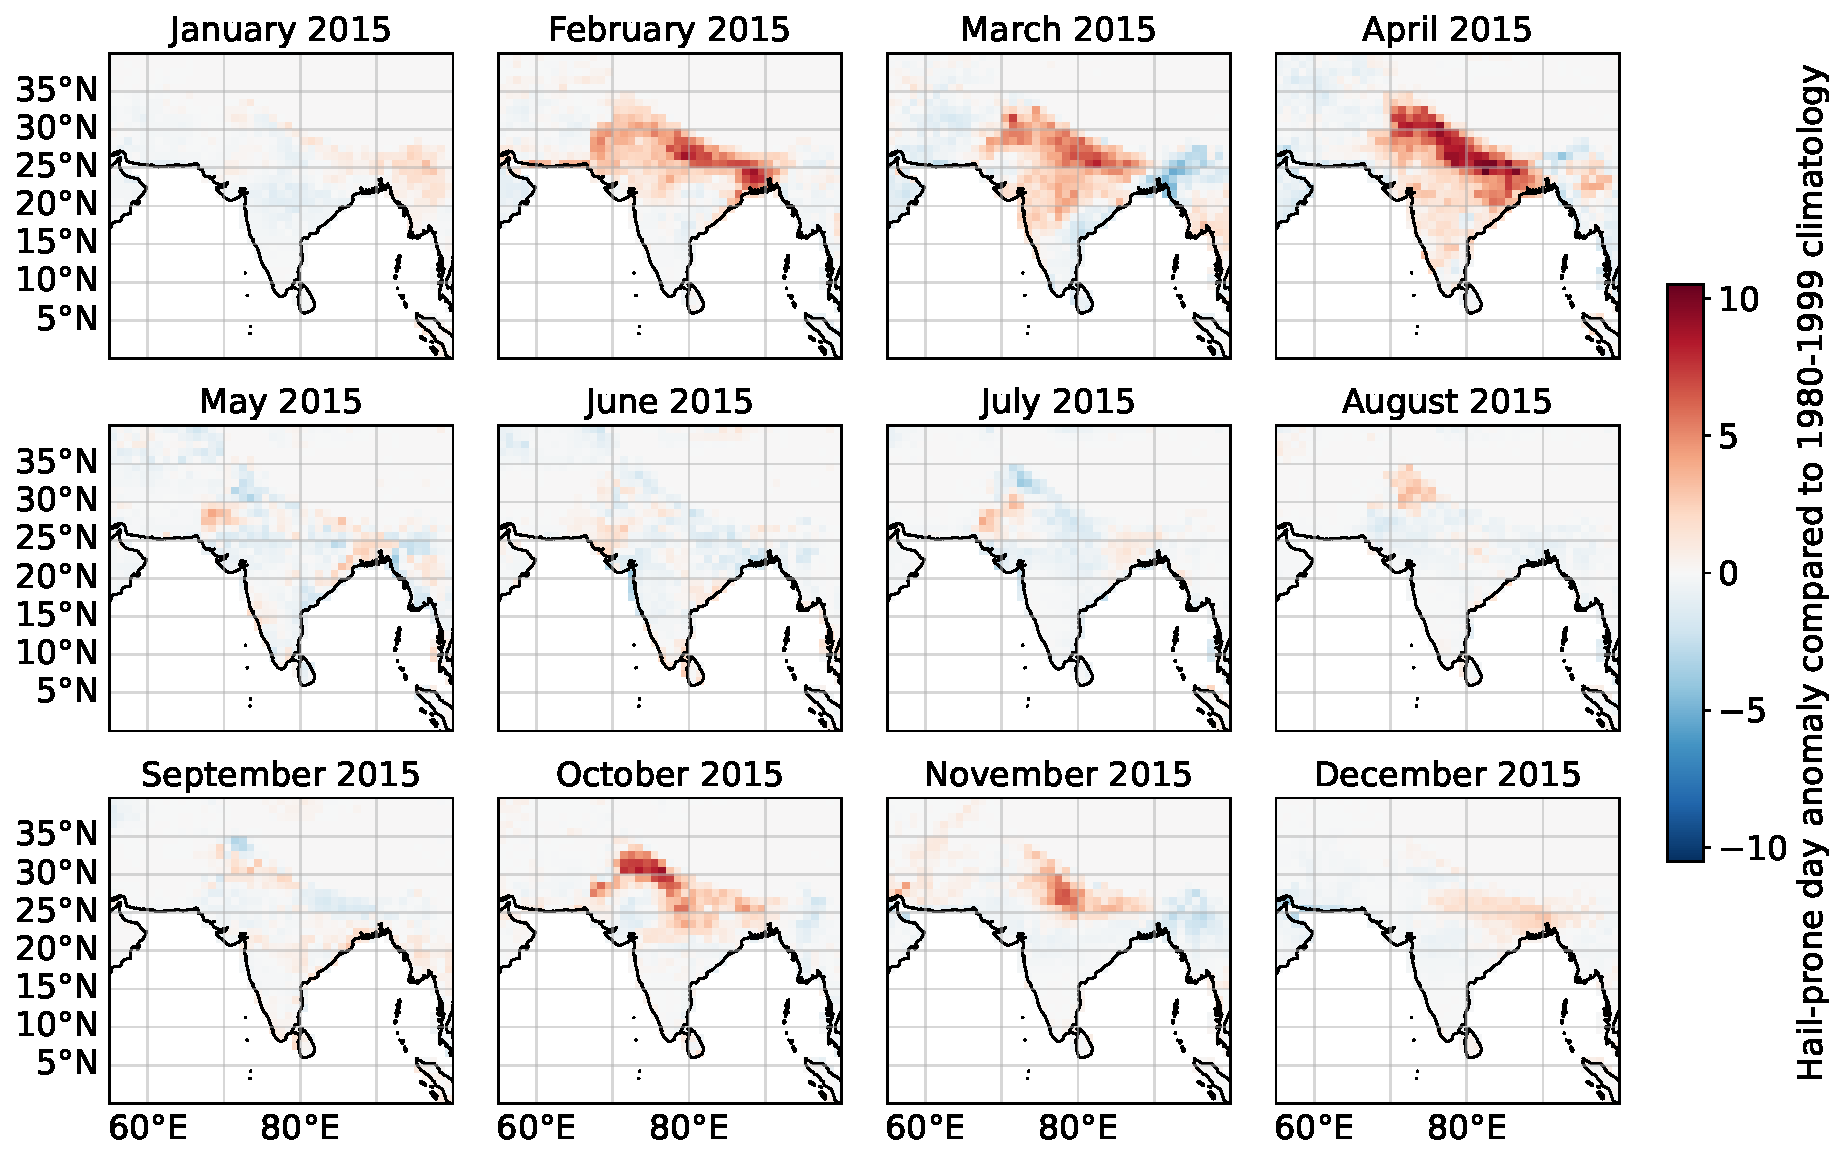
\includegraphics[width=\textwidth]{../../results/supplementary/monthly_anoms_India_2015}
    \caption{\textbf{Monthly multi-proxy mean normalised hail-prone day
    anomalies for the Indian region in 2015.} Anomalies are calculated using
    ERA5 data with respect to the monthly ERA5 historical climatology
    (1980-1999), figure shows multi-proxy mean anomalies. The normalisation
    factor was held constant.}
    \label{fig:anoms_India_2015}
\end{figure*}

\begin{figure*}[h]
    \centering
    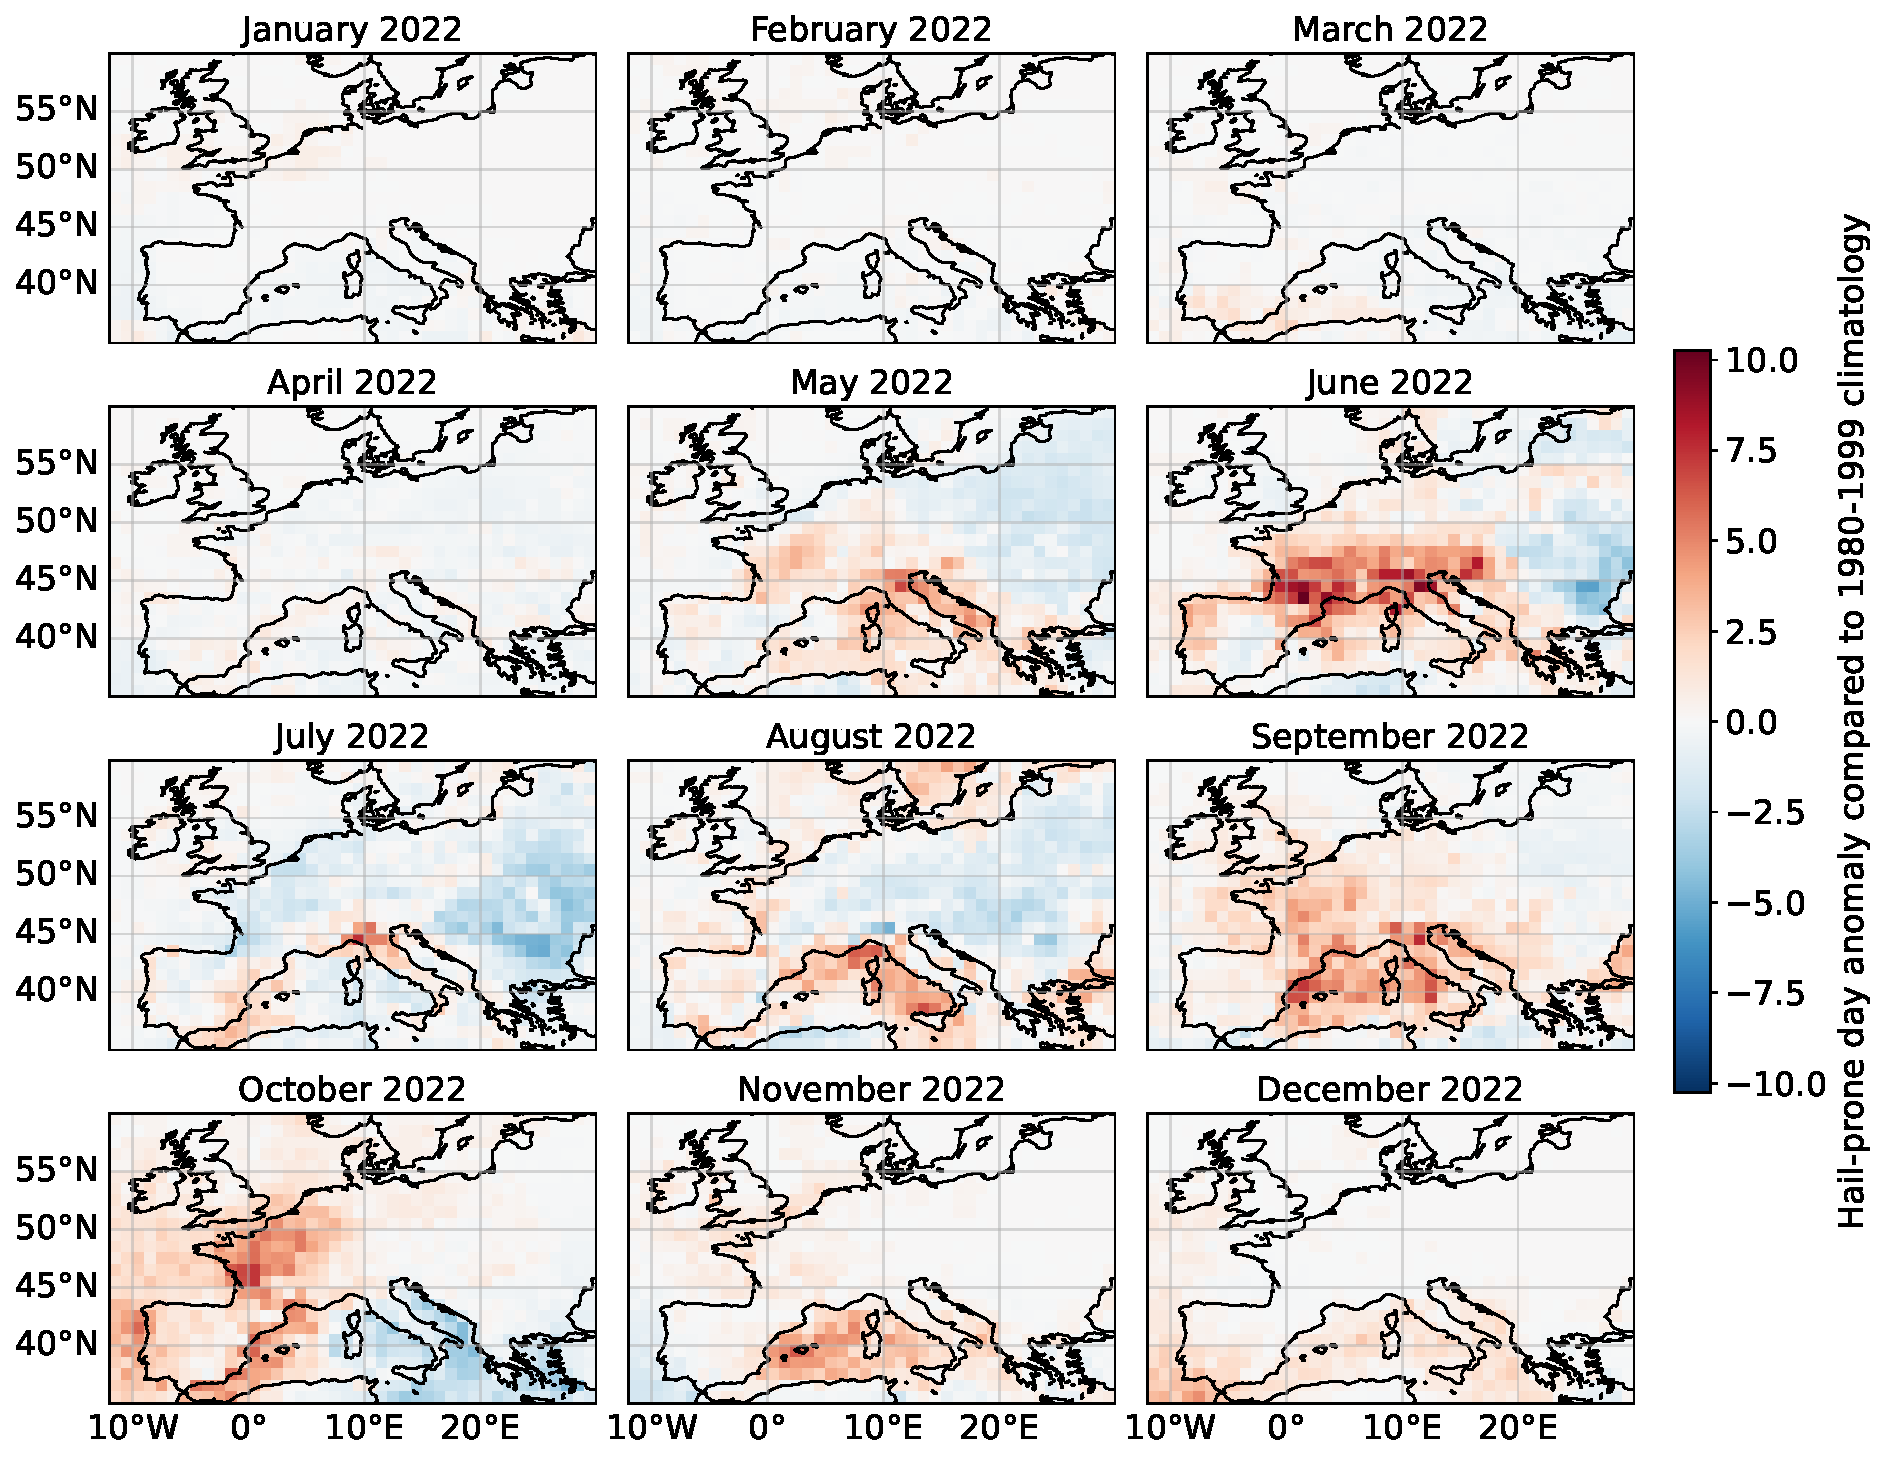
\includegraphics[width=\textwidth]{../../results/supplementary/monthly_anoms_France_2022}
    \caption{As for Supplementary Figure \ref{fig:anoms_India_2015} but for
    Europe in 2022.}
    \label{fig:anoms_Europe_2022}
\end{figure*}

\begin{figure*}[h]
    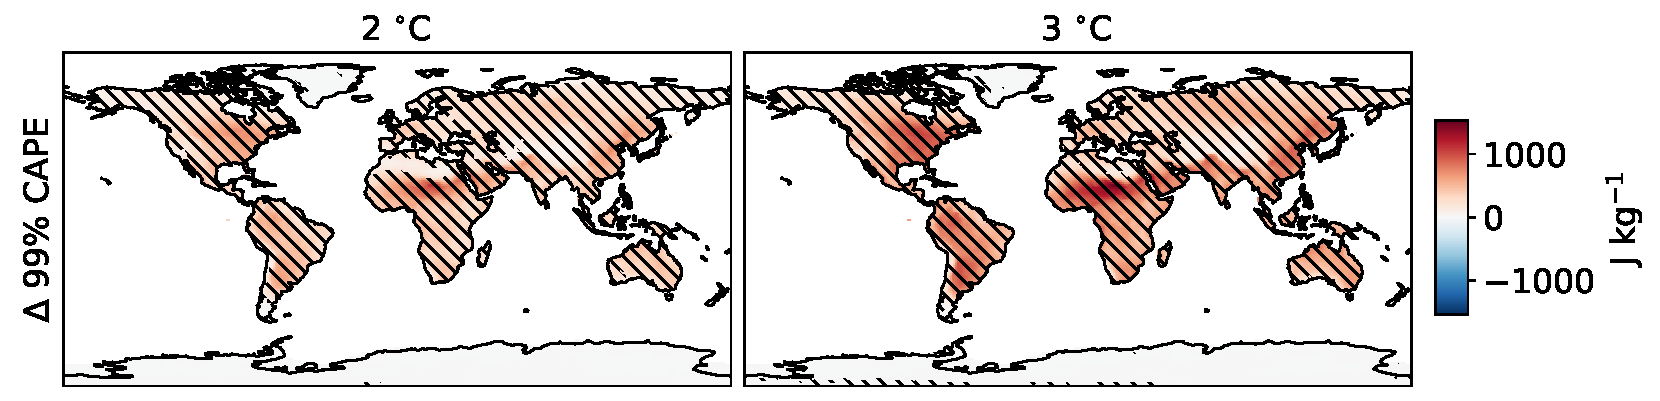
\includegraphics[width=\textwidth]{../../results/supplementary/ingredients_changes_cape}
    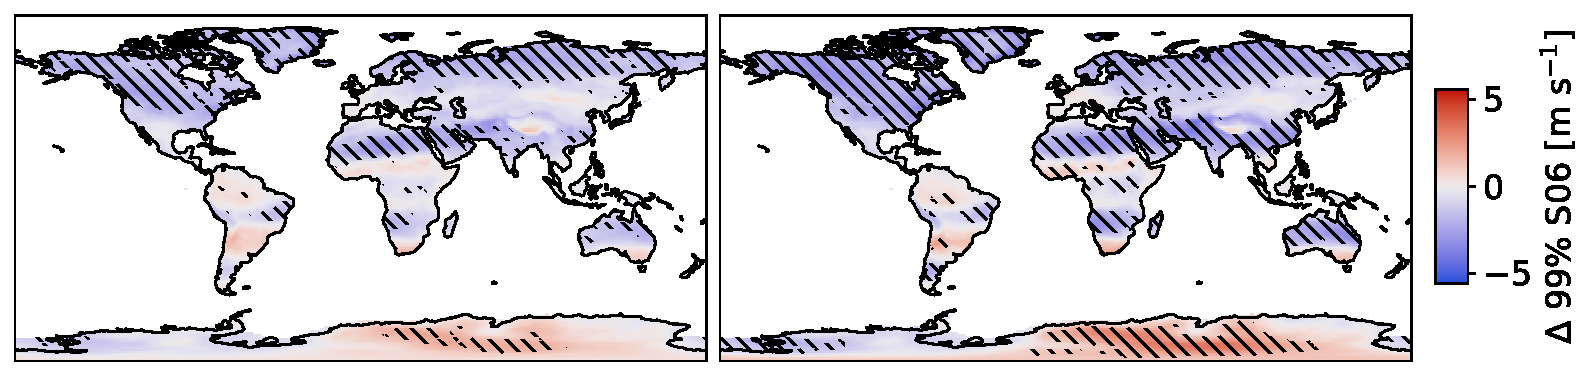
\includegraphics[width=0.958\textwidth]{../../results/supplementary/ingredients_changes_shear}
    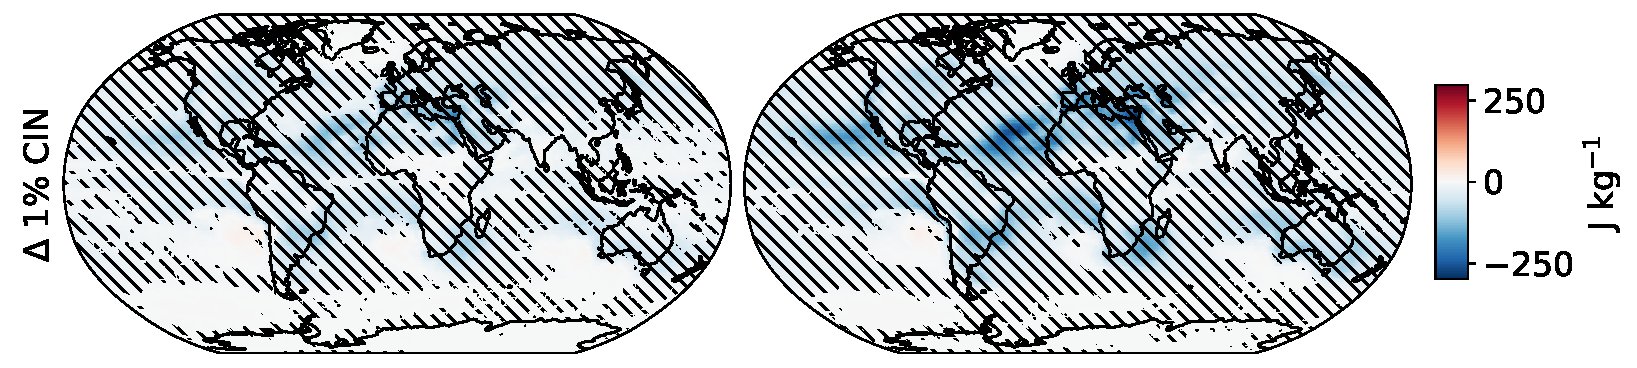
\includegraphics[width=0.987\textwidth]{../../results/supplementary/ingredients_changes_cin}
    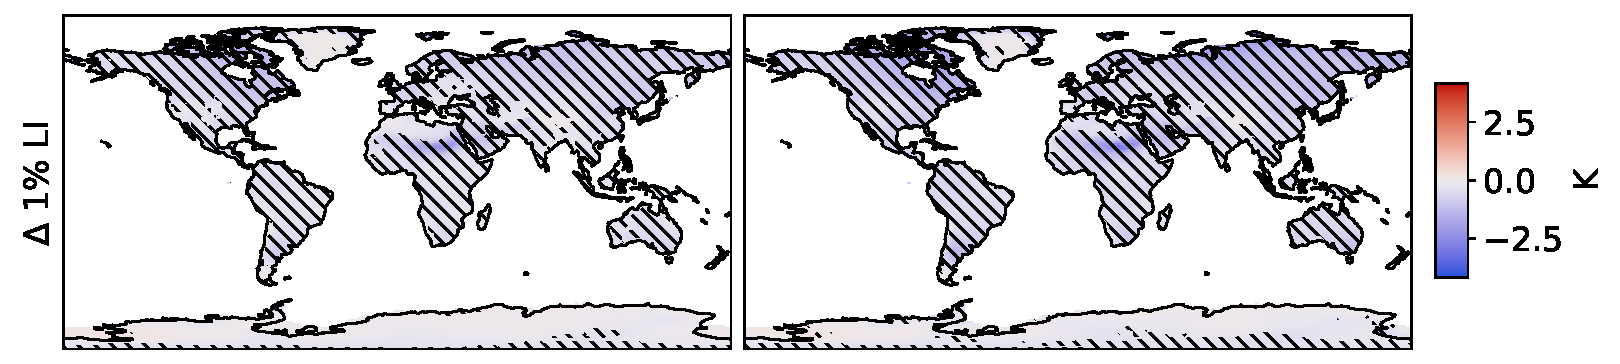
\includegraphics[width=0.976\textwidth]{../../results/supplementary/ingredients_changes_lifted_index}
    \caption{\textbf{Multimodel mean differences in hail ingredients by epoch.}
    Ingredients shown are annual extreme (99th percentile) convective available
    potential energy (CAPE), annual extreme (99th percentile) 0-6 km bulk wind
    shear (S06), annual extreme (1st percentile) convective inhibition (CIN),
    and annual extreme (1st percentile) lifted index. CAPE, CIN, and LI were
    calculated using a well-mixed parcel over the lowest 100 hPa. Stippling
    shows regions in which at least 50\% of the model/proxy combinations agreed
    with the sign of the mean difference and also showed significant differences
    in the mean ($p < 0.05$ on a t-test on two related samples).}
    \label{fig:ingredients_changes_1}
\end{figure*}

\begin{figure*}[h]
    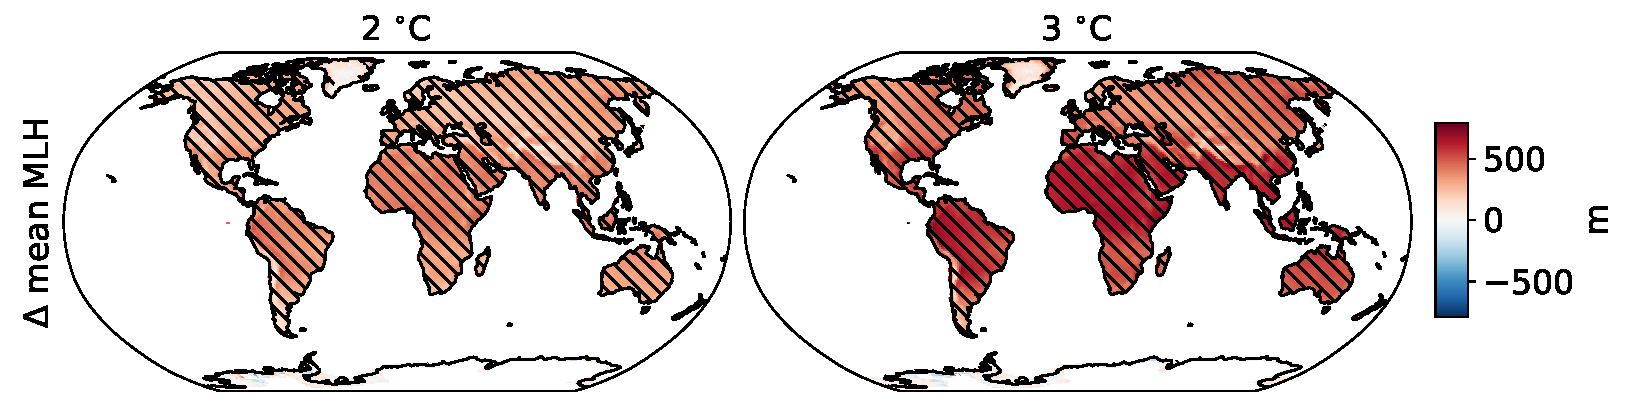
\includegraphics[width=0.955\textwidth]{../../results/supplementary/ingredients_changes_mlh}
    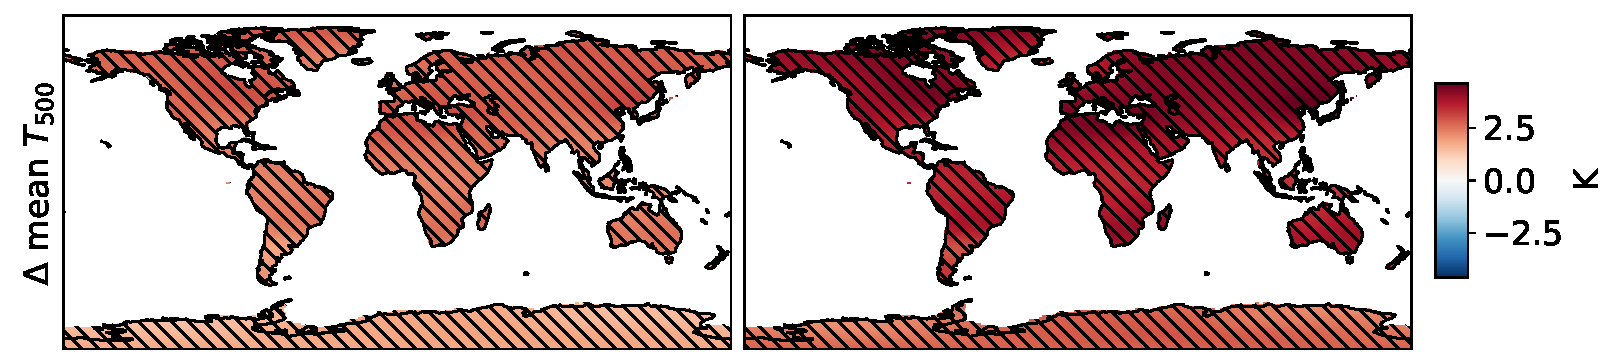
\includegraphics[width=0.955\textwidth]{../../results/supplementary/ingredients_changes_temp}
    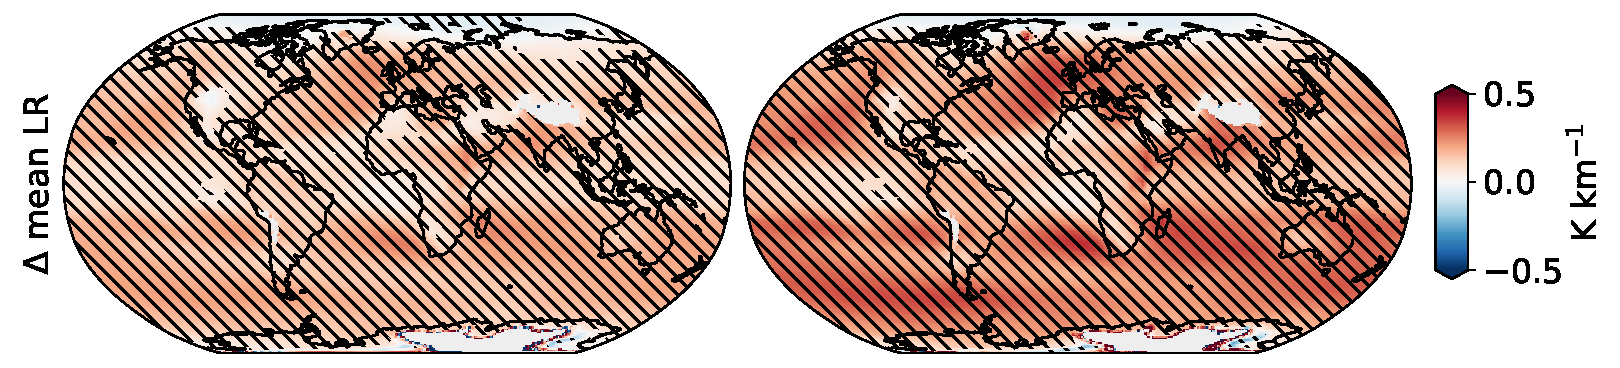
\includegraphics[width=0.955\textwidth]{../../results/supplementary/ingredients_changes_lapse_rate}
    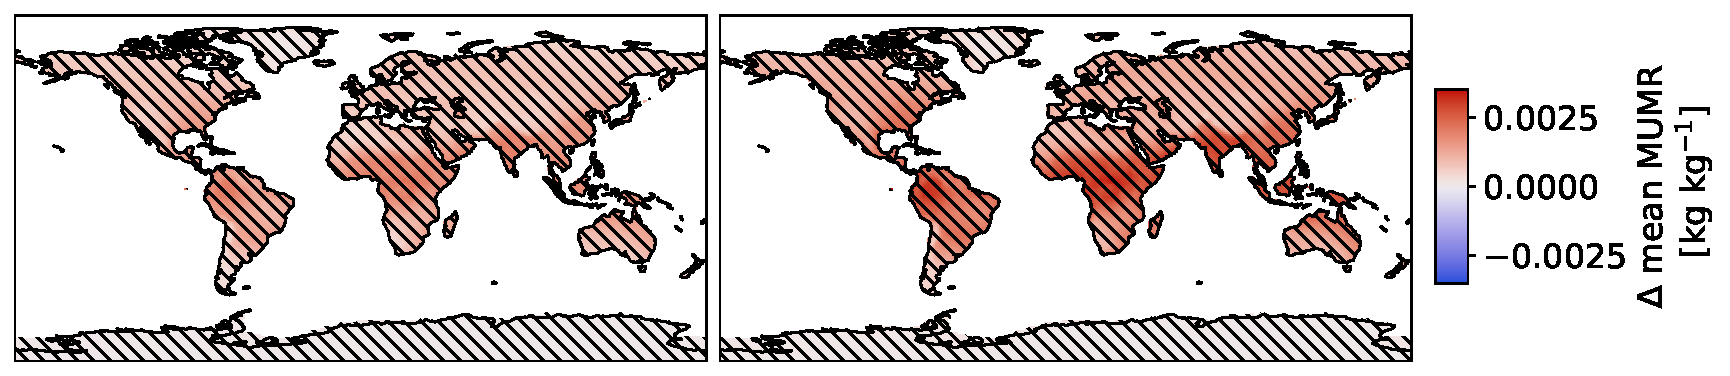
\includegraphics[width=\textwidth]{../../results/supplementary/ingredients_changes_mumr}
    \caption{As for Supplementary Figure \ref{fig:ingredients_changes_1} but for
    annual mean melting level height (MLH), annual mean temperature at 500 hPa
    ($T_{500}$), annual mean lapse rate (LR), and most-unstable parcel mixing
    ratio (MUMR). To increase contrast the colour scale for LR is truncated.}
    \label{fig:ingredients_changes_2}
\end{figure*}

\begin{figure*}[h]
    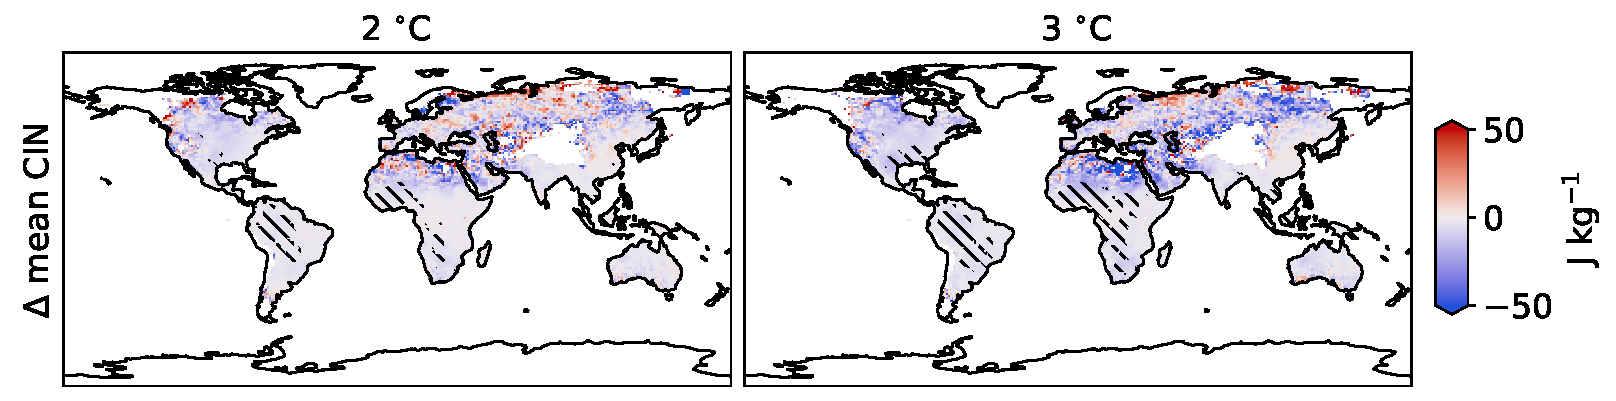
\includegraphics[width=0.981\textwidth]{../../results/supplementary/ingredients_changes_mlcin_extreme_cape}
    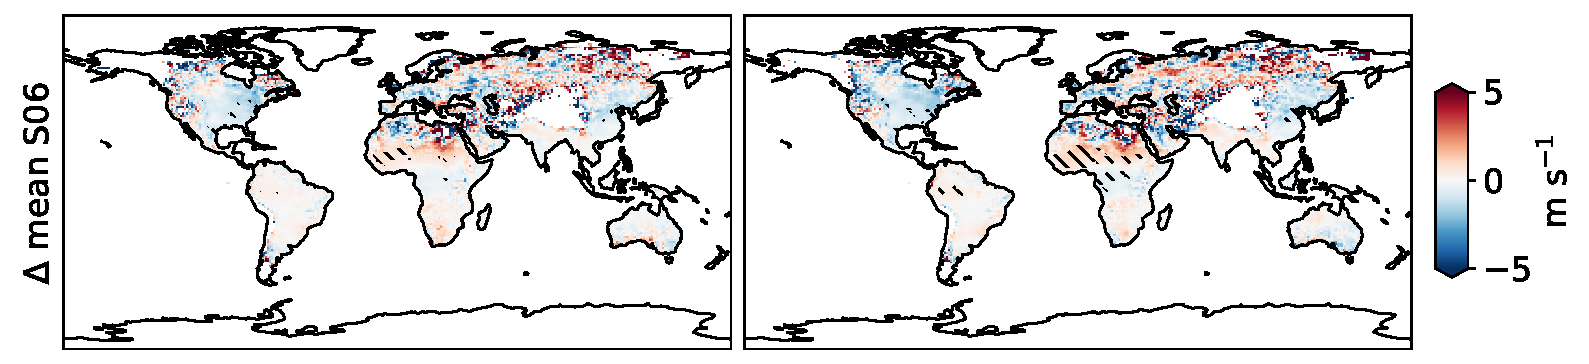
\includegraphics[width=0.963\textwidth]{../../results/supplementary/ingredients_changes_shear_extreme_cape}
    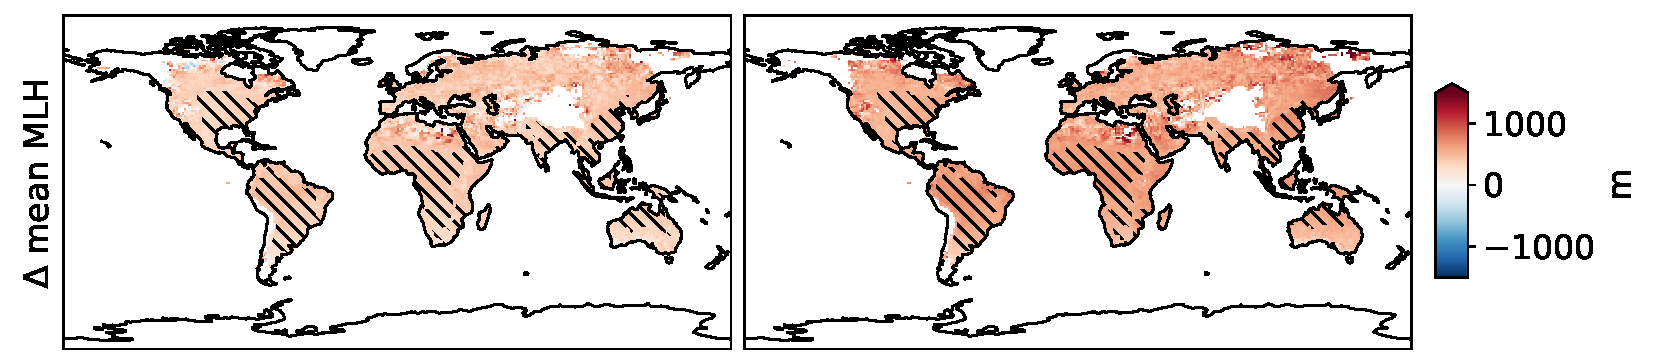
\includegraphics[width=\textwidth]{../../results/supplementary/ingredients_changes_mlh_extreme_cape}
    \caption{As for Supplementary Figure \ref{fig:ingredients_changes_1} but
    showing changes in annual mean CIN, S06, and melting level height (MLH),
    only for times and locations when CAPE is over the 99th percentile
    calculated for each epoch.}
    \label{fig:ingredients_changes_at_extreme_times}
\end{figure*}

\begin{figure*}[h]
    \centering
    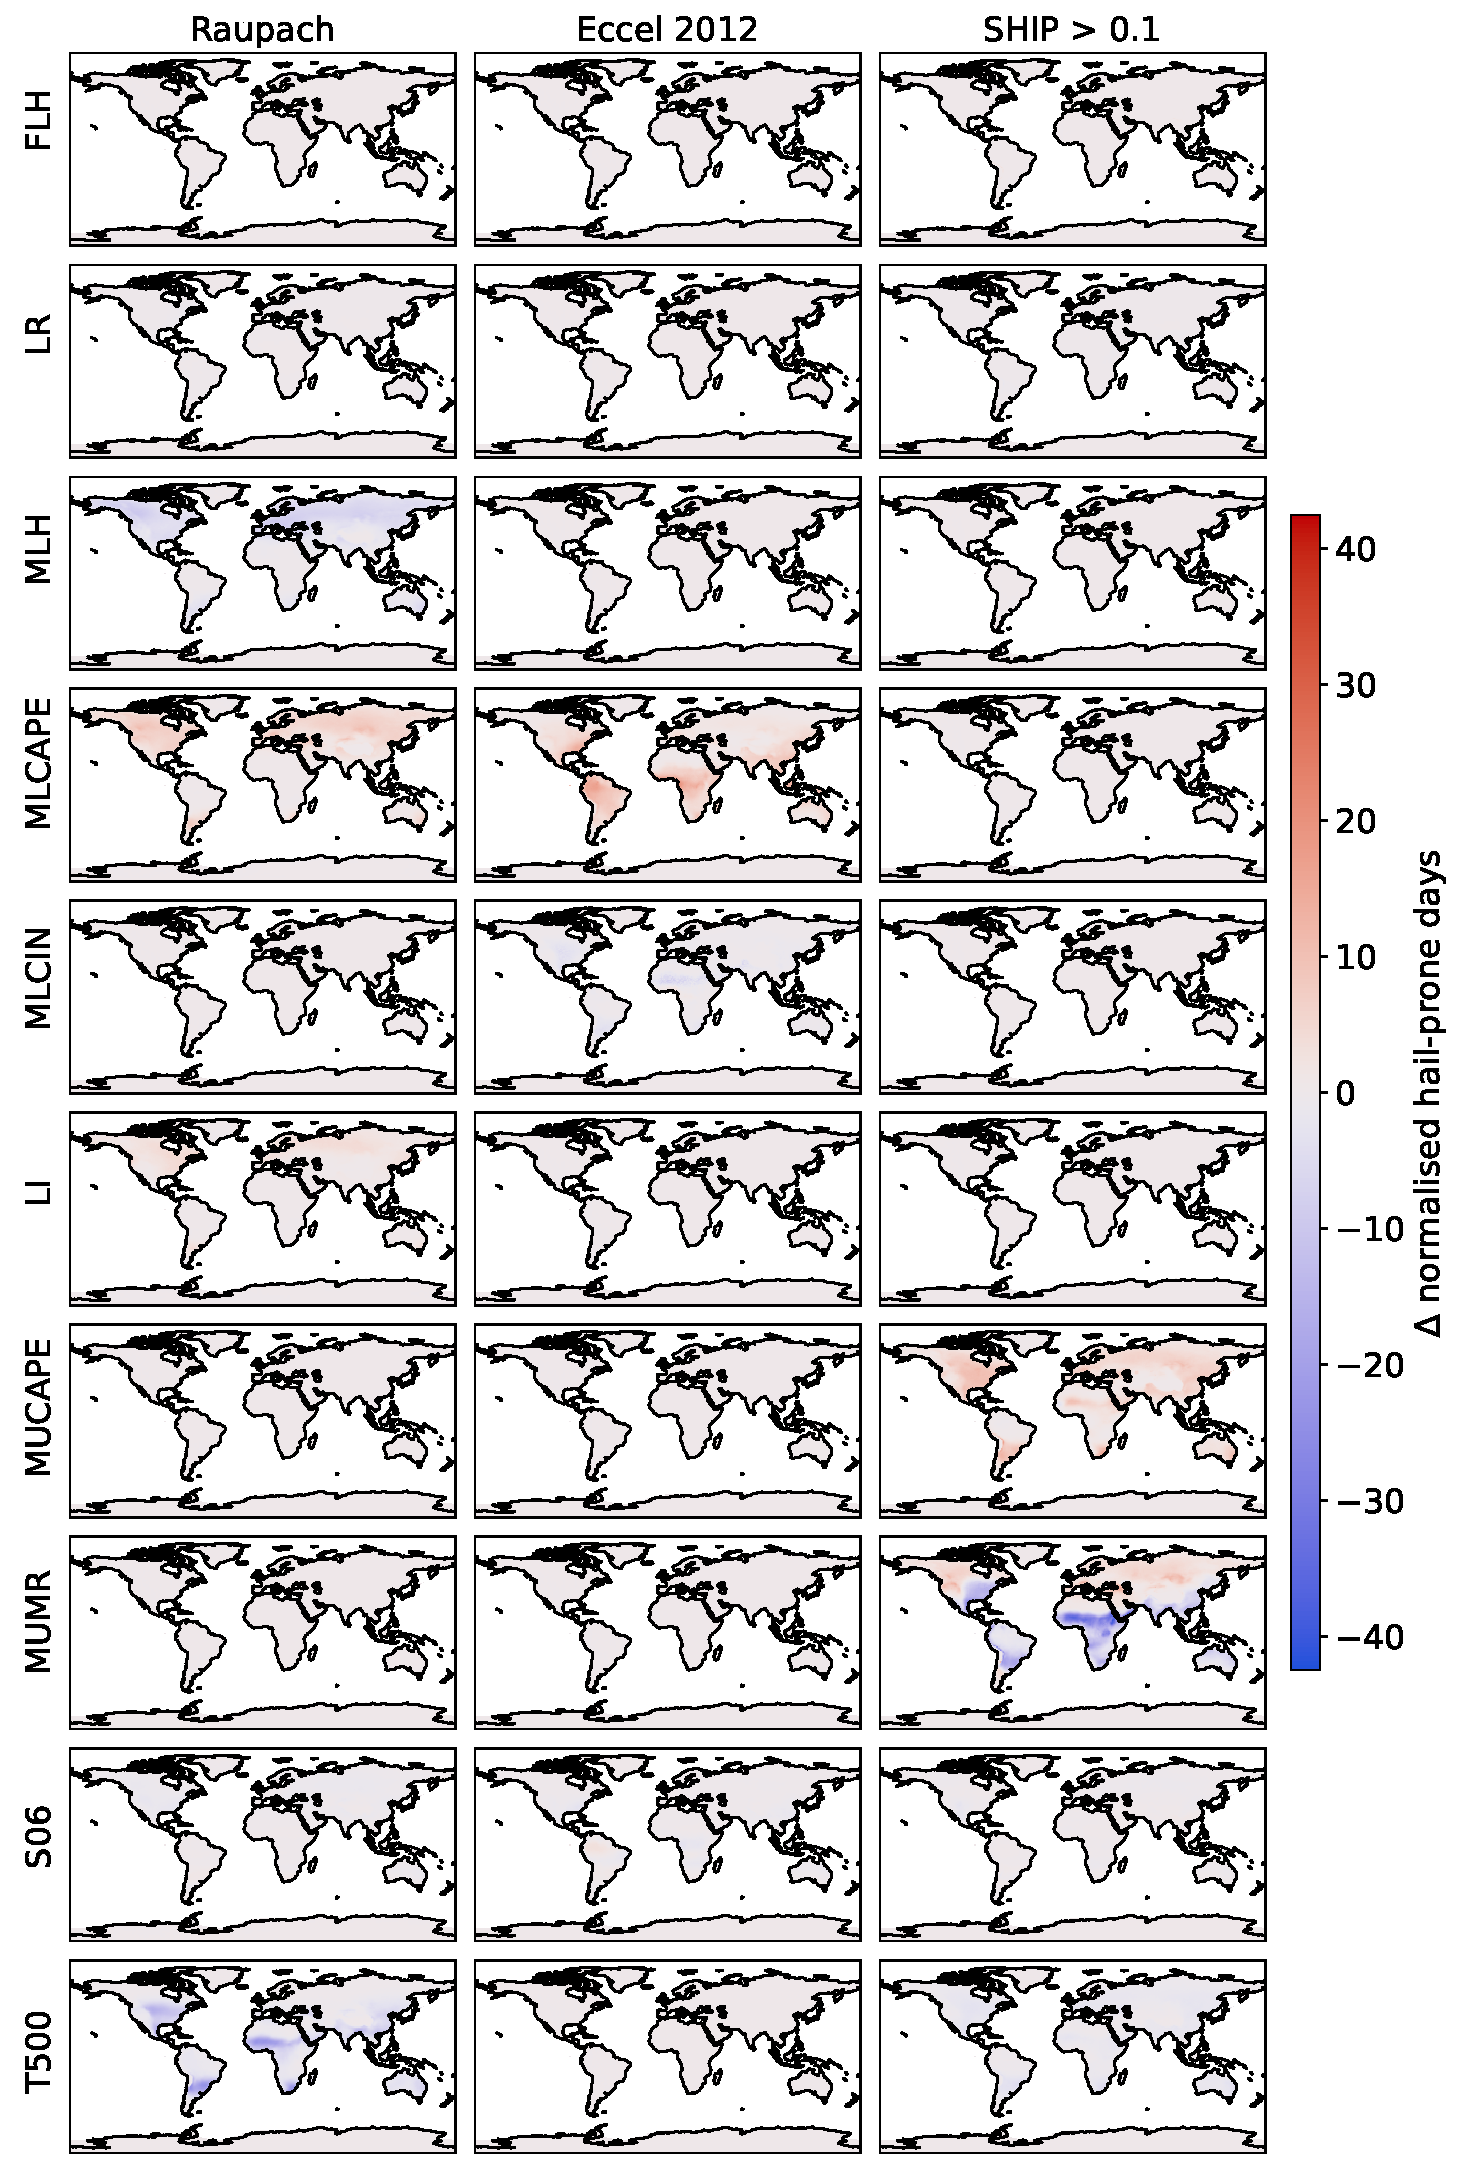
\includegraphics[width=0.81\textwidth]{../../results/supplementary/all_drivers}
    \caption{\textbf{Drivers of changes across models.} Rows show de-biased
    ingredients: freezing level height (FLH), lapse rate (LR), melting level
    height (MLH), mixed-layer CAPE (MLCAPE$_{100}$), mixed-layer CIN
    (MLCIN$_{100}$), lifted index (LI), most-unstable CAPE (MUCAPE$_{250}$),
    most-unstable mixing ratio (MUMR), 0-6 km bulk shear (S06), and temperature
    at 500 hPa (T500).}
    \label{fig:drivers}
\end{figure*}

\begin{figure*}[h]
    \centering
    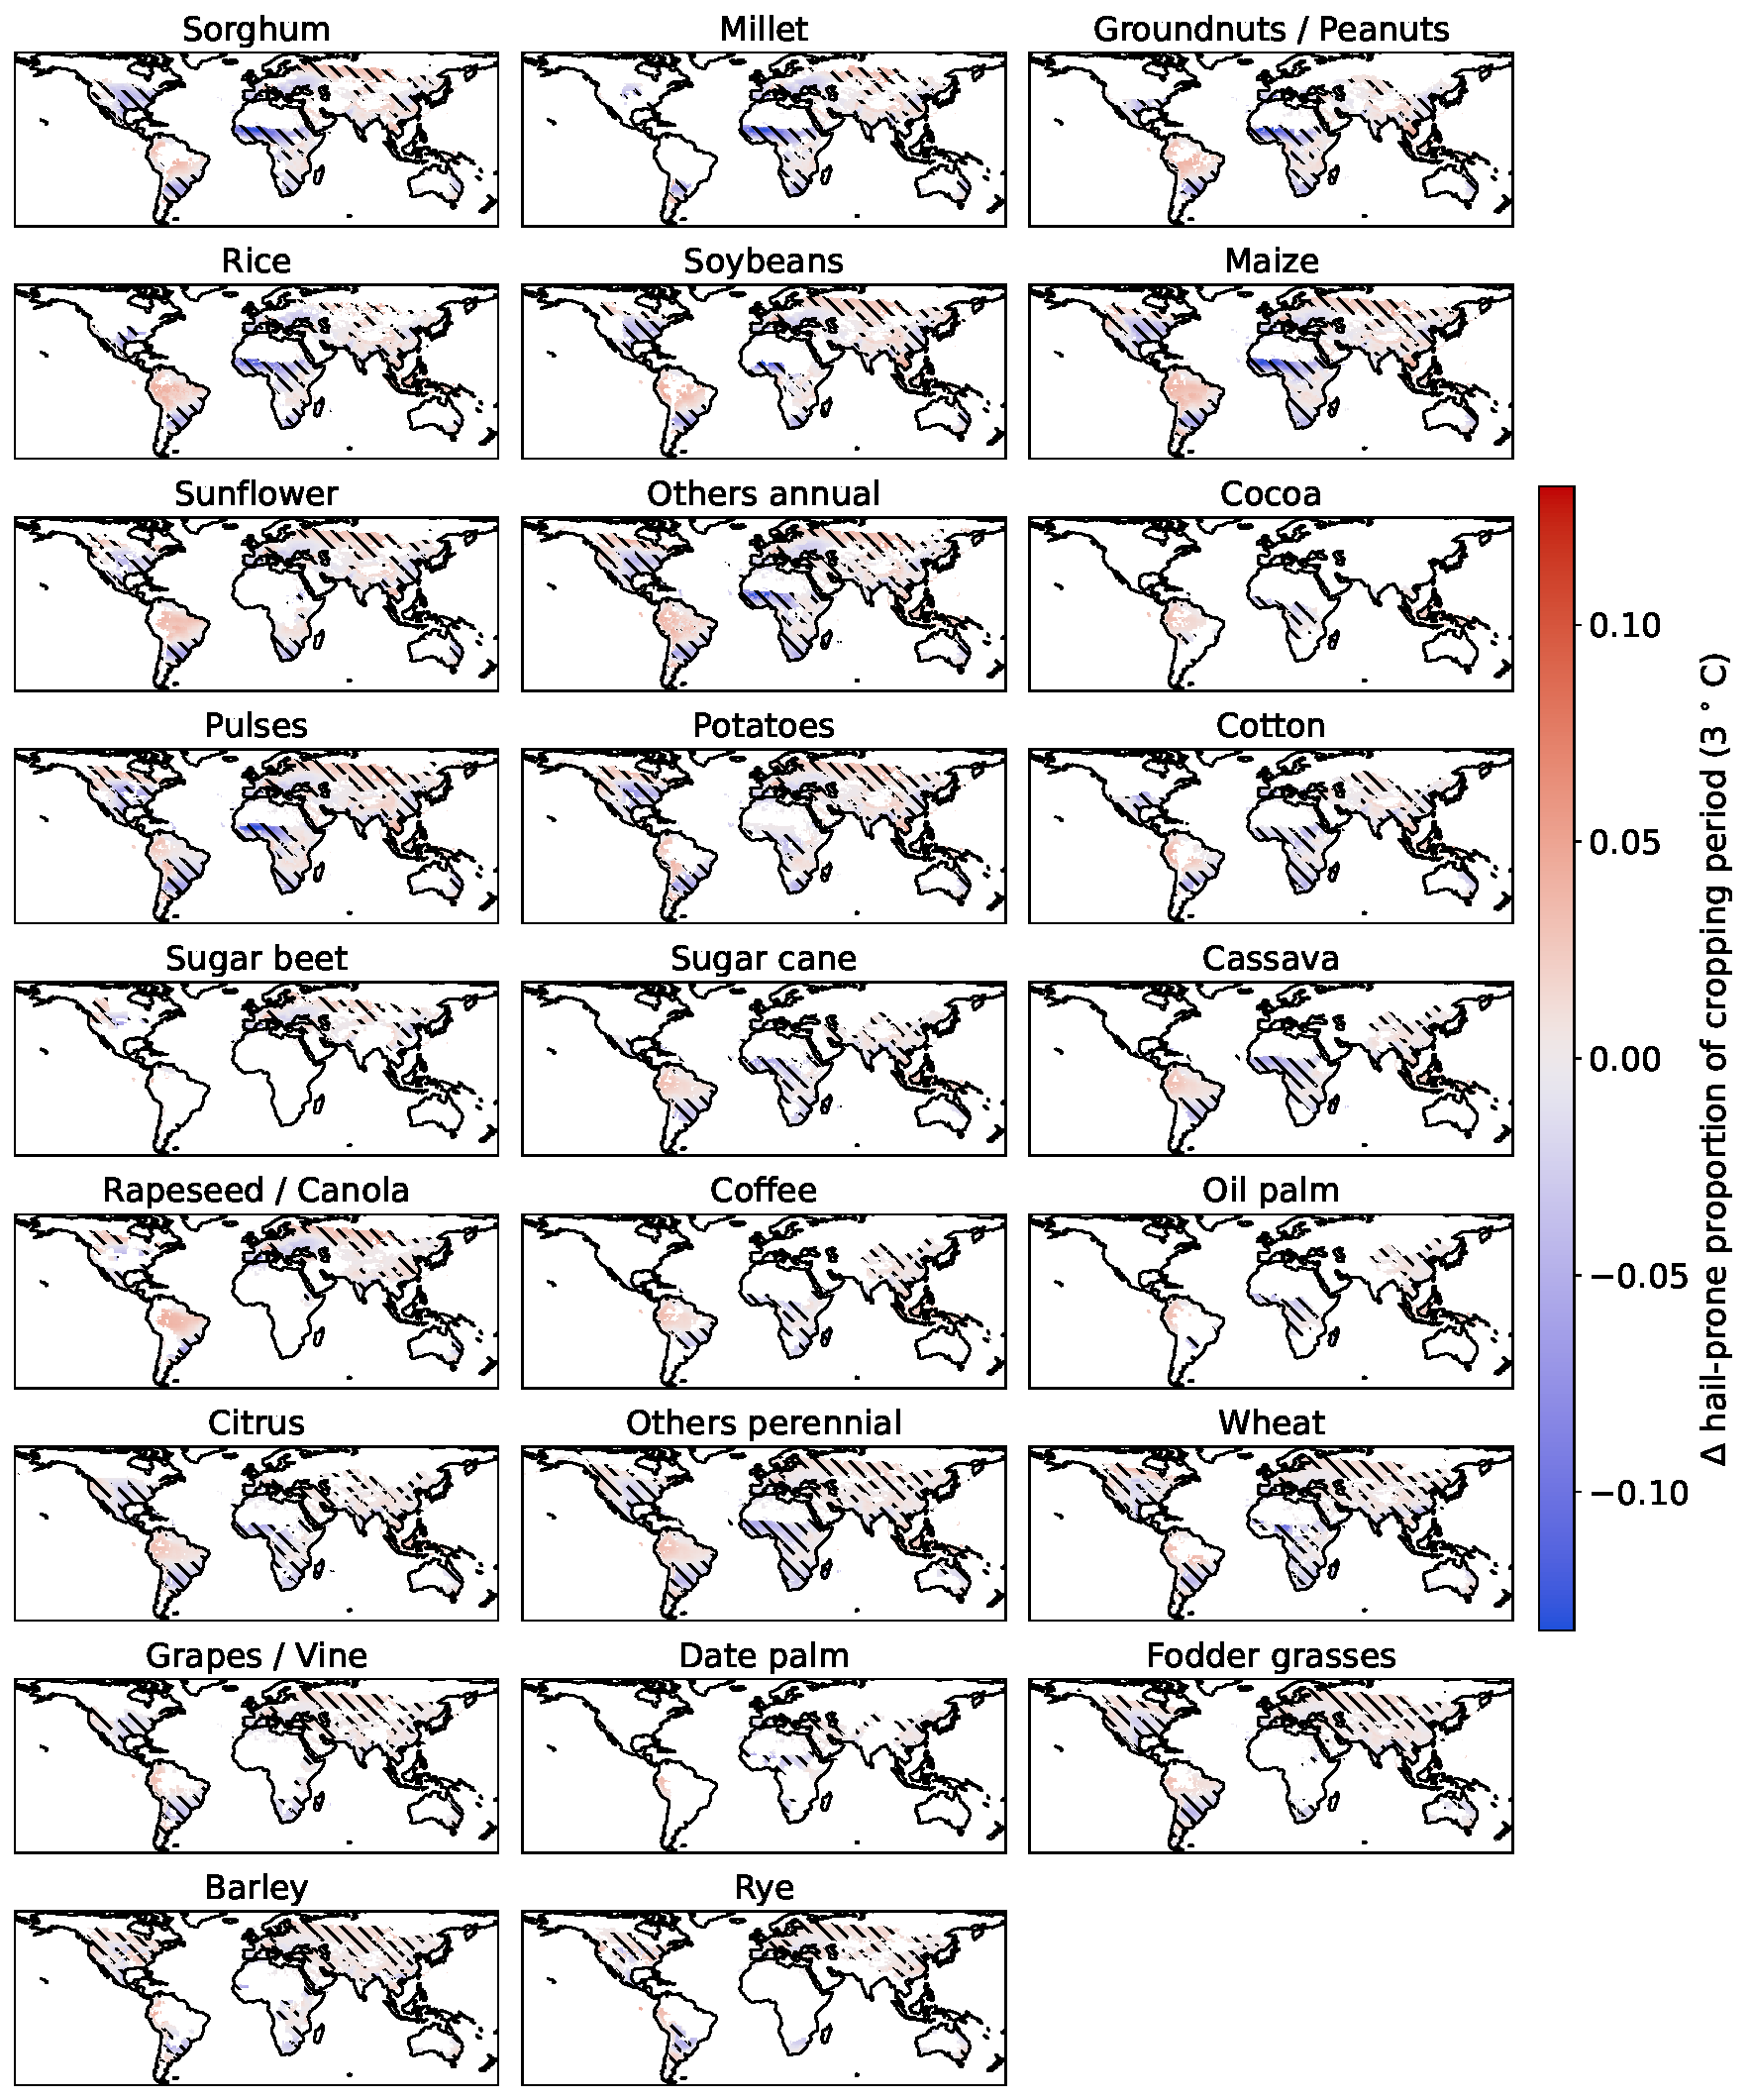
\includegraphics[width=\textwidth]{../../results/supplementary/changes_crop_proportion_hail_prone_3C}
    \caption{\textbf{Multimodel, multi-proxy mean change in hail-prone
    proportions of cropping seasons for 3 \degr{} warming.} Stippling as for
    Supplementary Figure \ref{fig:ingredients_changes_1} and region subset as
    for Extended Data Figure \ref{ED-fig:historic_crop_proportions}.}
    \label{fig:crop_changes_3C}
\end{figure*}

\begin{figure*}[h]
    \centering
    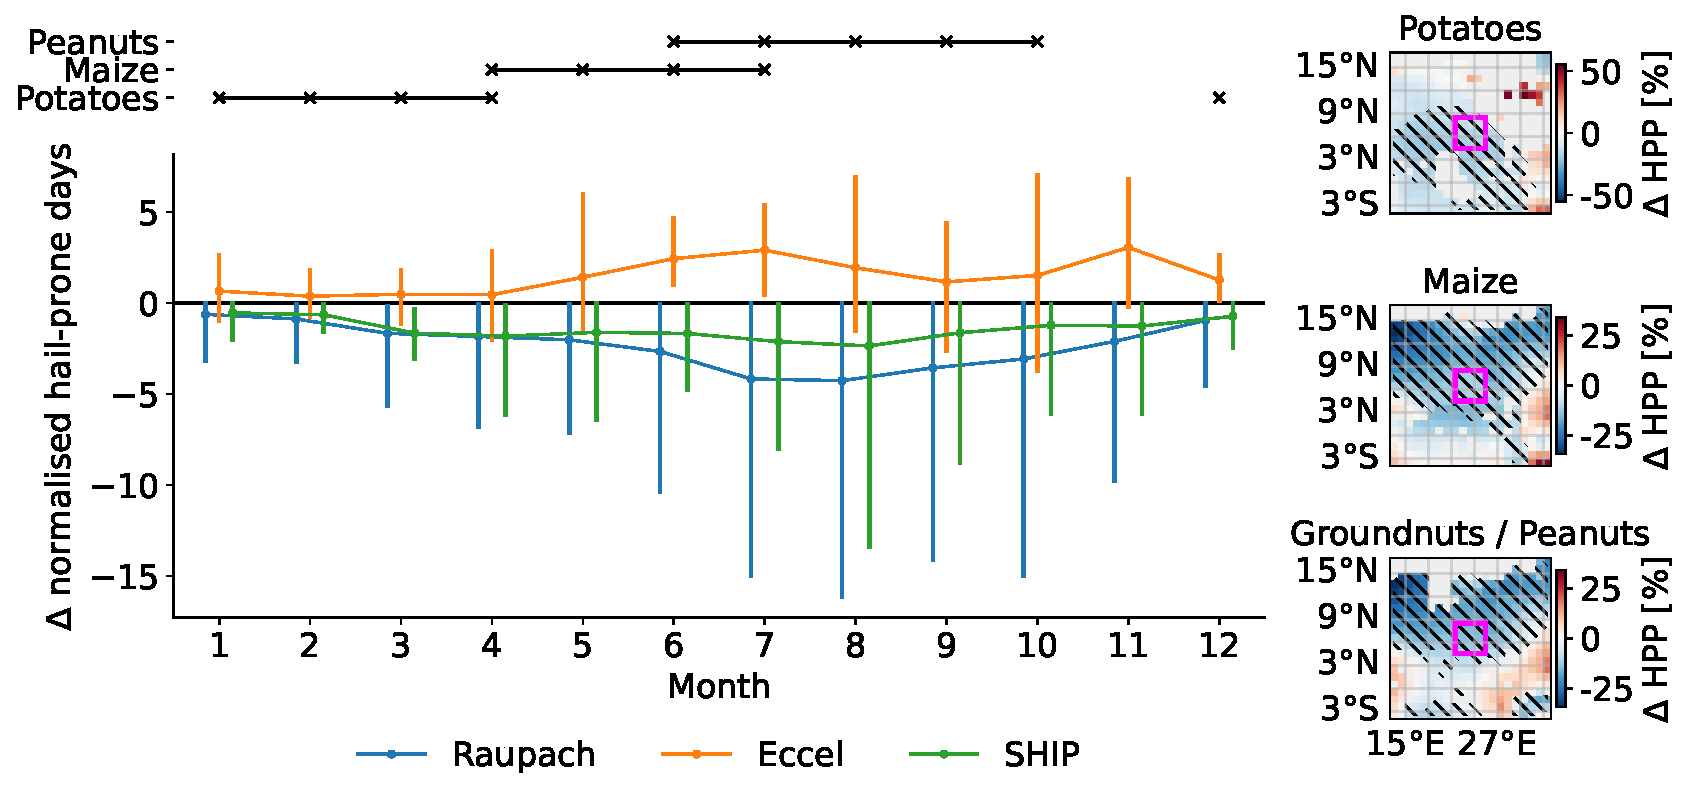
\includegraphics[width=\textwidth]{../../results/supplementary/crop_lines_af}
    \caption{\textbf{Changes affecting crops at a selected location in Africa.}
    The horizontal black lines in the top inset plot indicate which months are
    considered cropping times for selected crops at the given location. The
    chosen location is at the centre of the fuchsia square in the inset maps.
    Inset maps show changes in hail-prone proportion of cropping season by crop.
    Lines in main plot show mean changes in hail-prone days per month over a
    4$\times$4\degr{} region around the chosen location (shown as a fuchsia
    square in inset maps), with vertical lines indicating the inter-model range
    per proxy. Stippling in inset maps as for Figure
    \ref{fig:ingredients_changes_1}.}
    \label{fig:crop_lines_af}
\end{figure*}

\begin{figure*}[h]
    \centering
    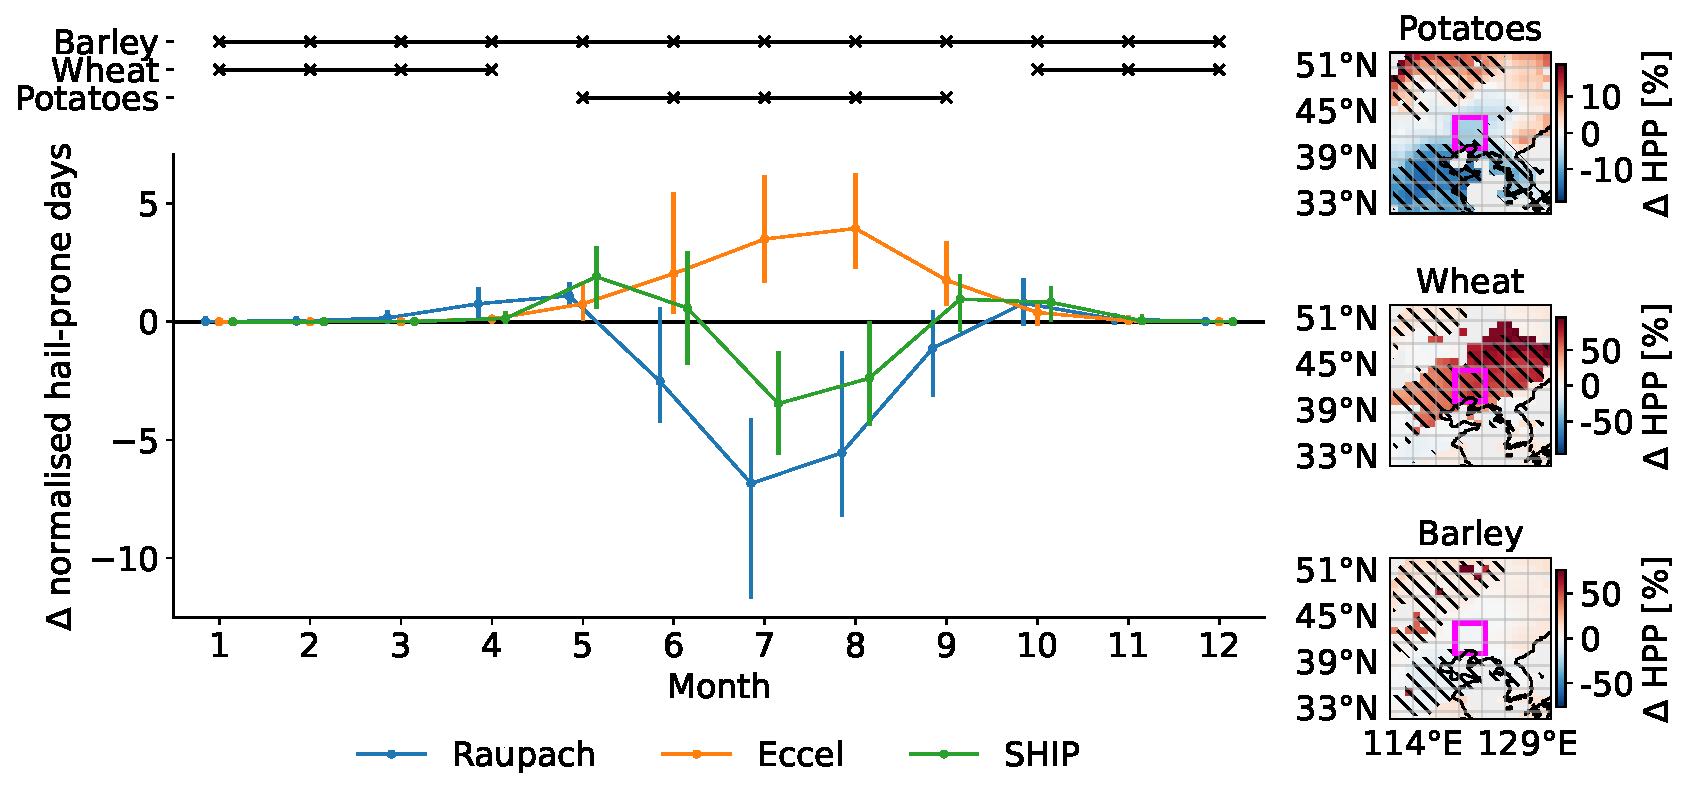
\includegraphics[width=\textwidth]{../../results/supplementary/crop_lines_as}
    \caption{As for Figure \ref{fig:crop_lines_af} but for Asia.}
    \label{fig:crop_lines_as}
\end{figure*}

\begin{figure*}[h]
    \centering
    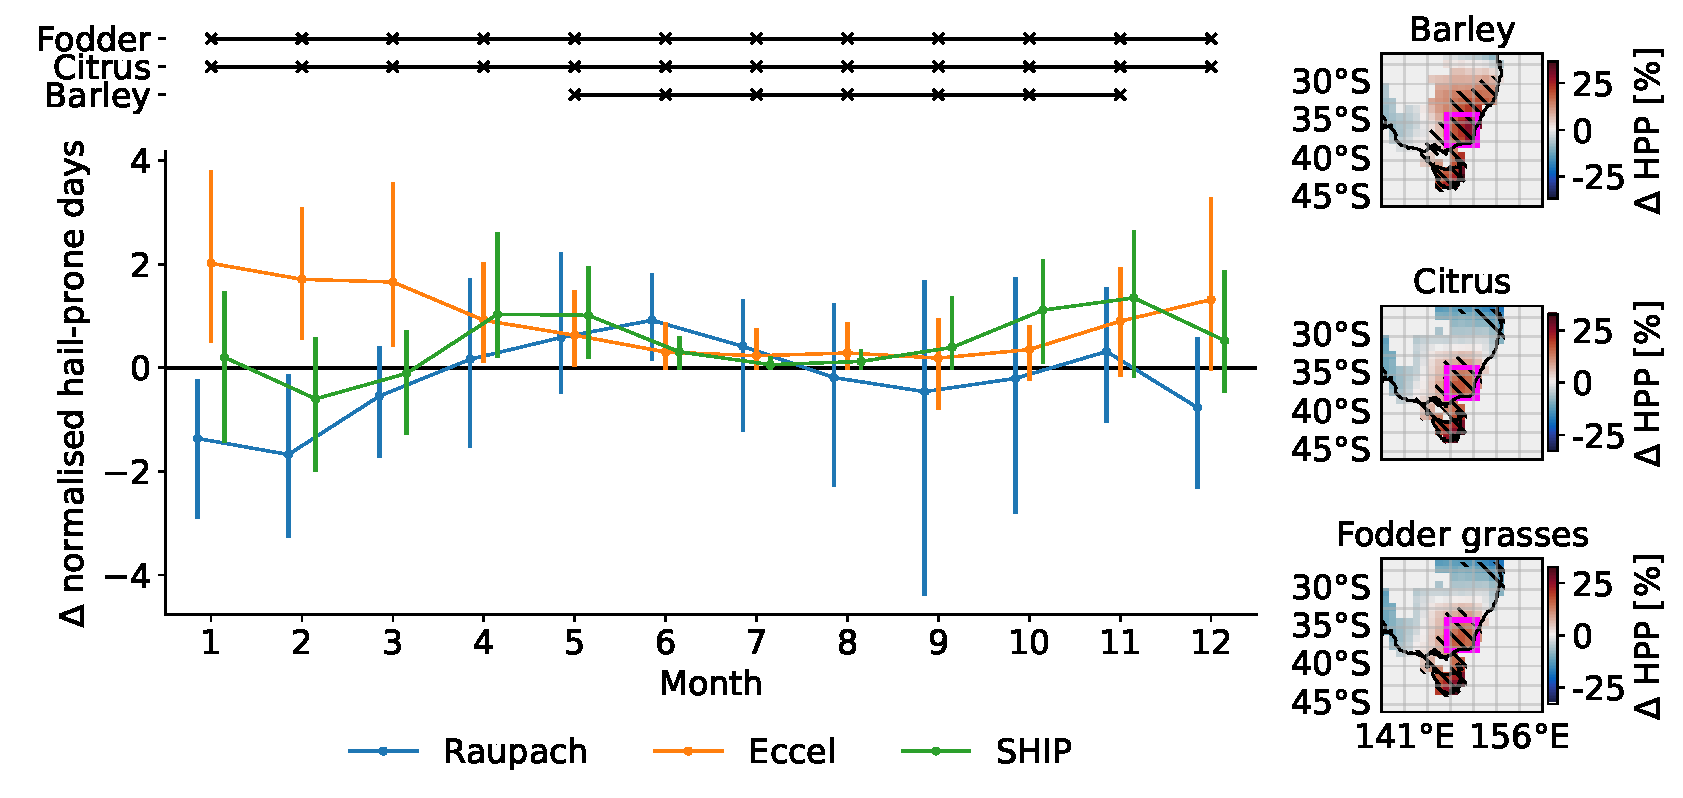
\includegraphics[width=\textwidth]{../../results/supplementary/crop_lines_au}
    \caption{As for Figure \ref{fig:crop_lines_af} but for Australia.}
    \label{fig:crop_lines_au}
\end{figure*}

\begin{figure*}[h]
    \centering
    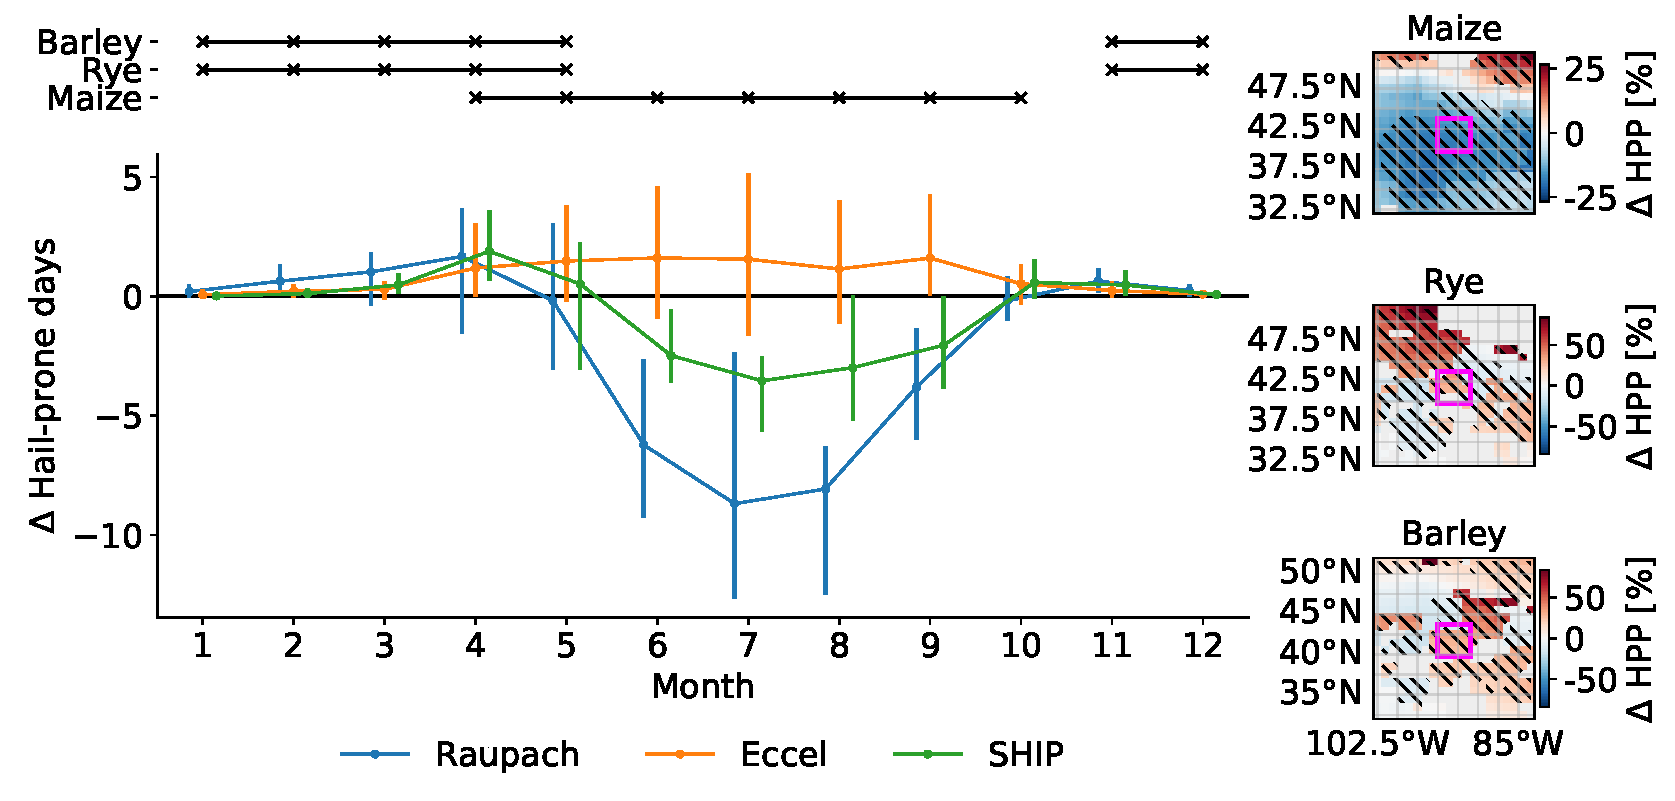
\includegraphics[width=\textwidth]{../../results/supplementary/crop_lines_us}
    \caption{As for Figure \ref{fig:crop_lines_af} but for the USA.}
    \label{fig:crop_lines_ca}
\end{figure*}

\begin{figure*}[h]
    \centering
    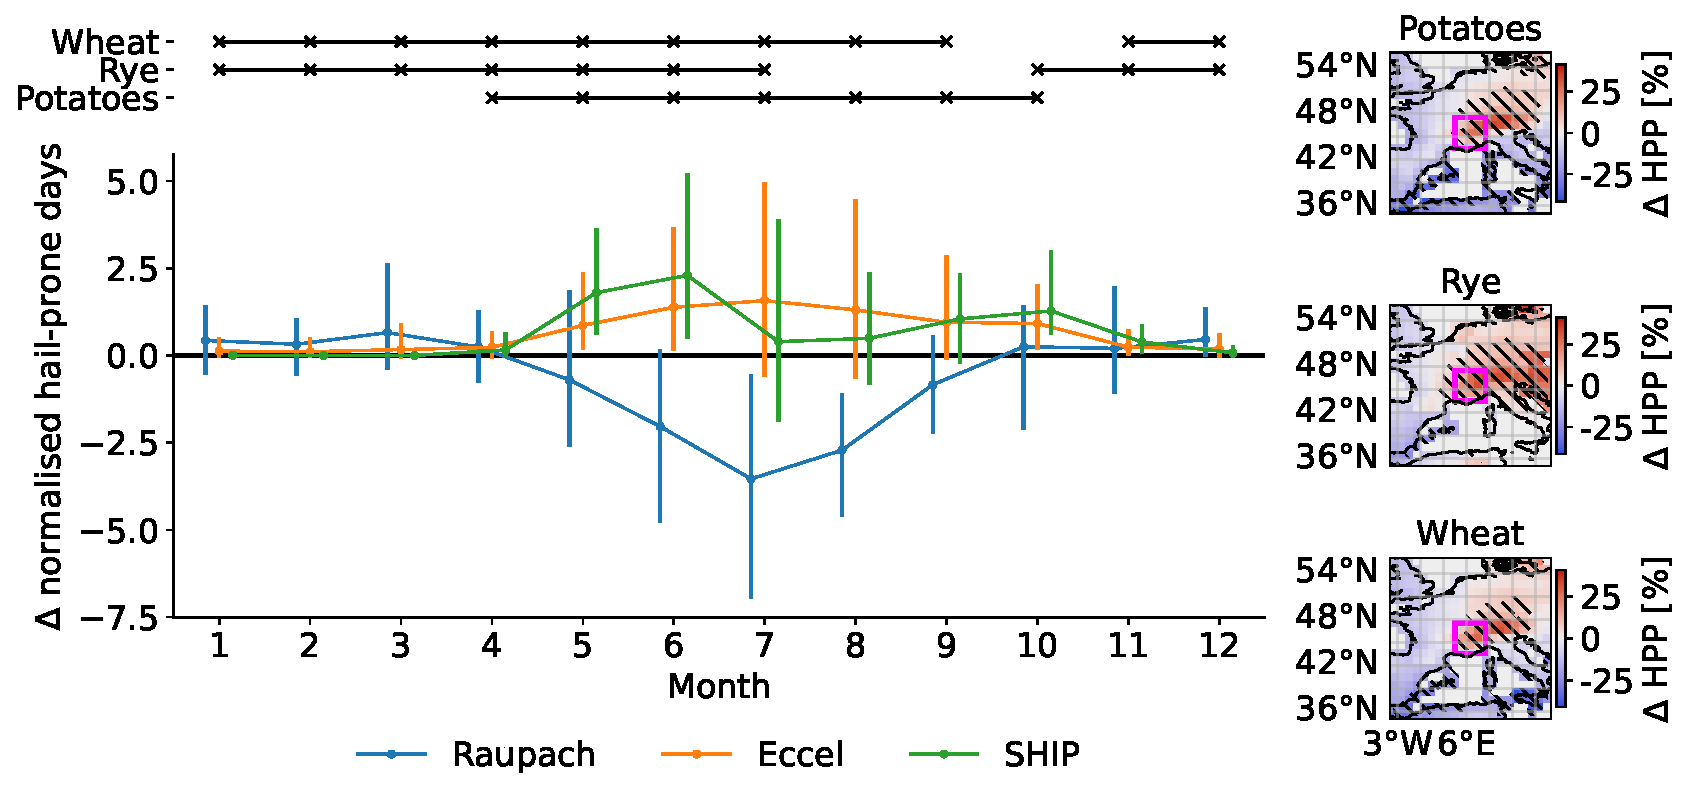
\includegraphics[width=\textwidth]{../../results/supplementary/crop_lines_eu}
    \caption{As for Figure \ref{fig:crop_lines_af} but for Europe.}
    \label{fig:crop_lines_eu}c
\end{figure*}

\begin{figure*}[h]
    \centering
    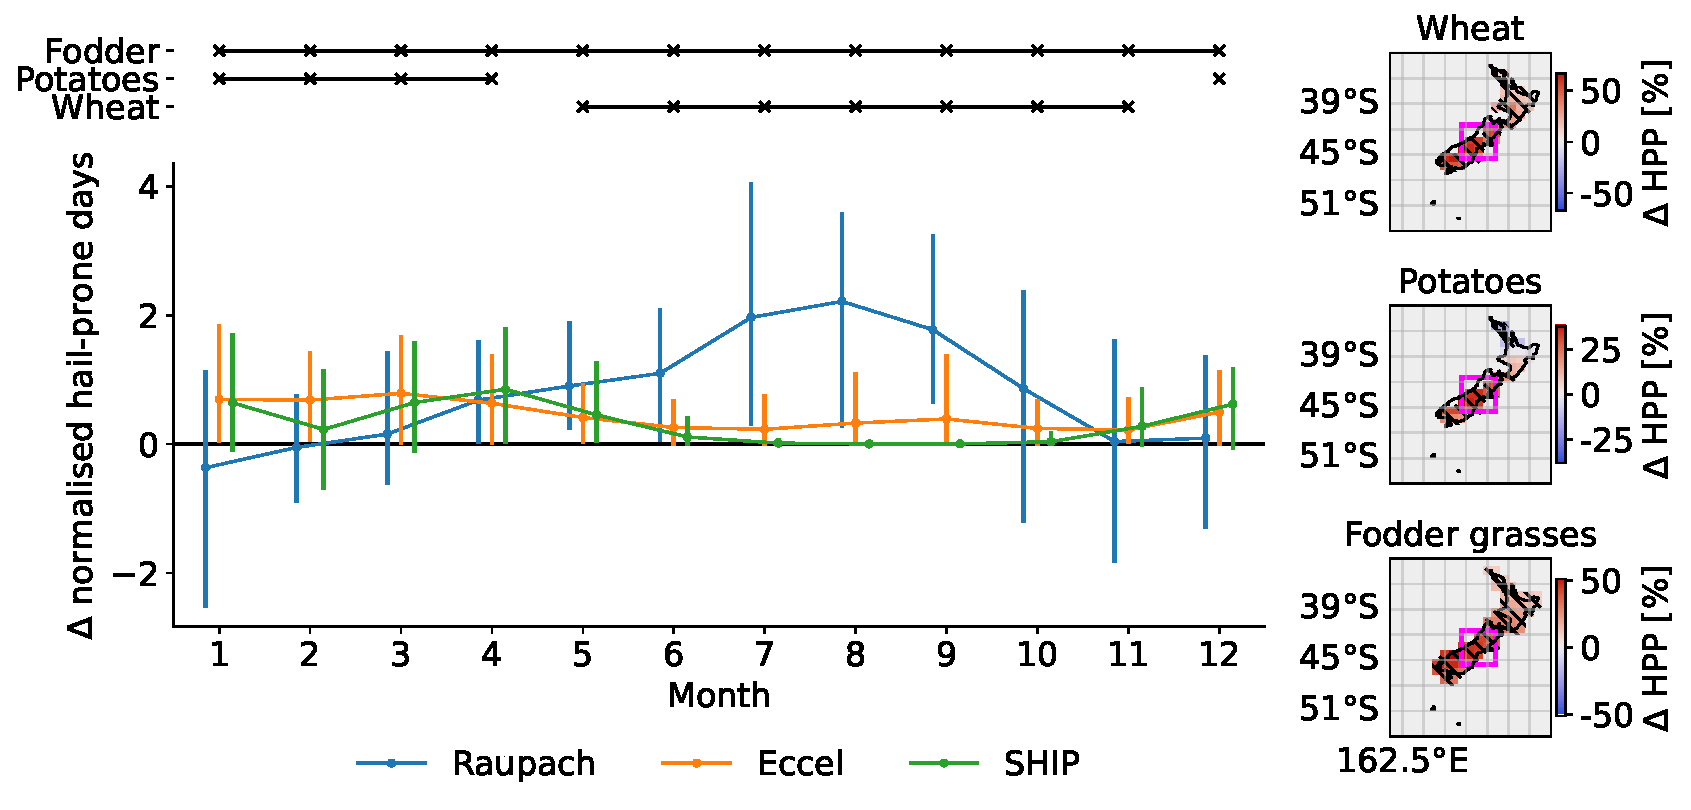
\includegraphics[width=\textwidth]{../../results/supplementary/crop_lines_nz}
    \caption{As for Figure \ref{fig:crop_lines_af} but for New Zealand.}
    \label{fig:crop_lines_nz}
\end{figure*}

\begin{figure*}[h]
    \centering
    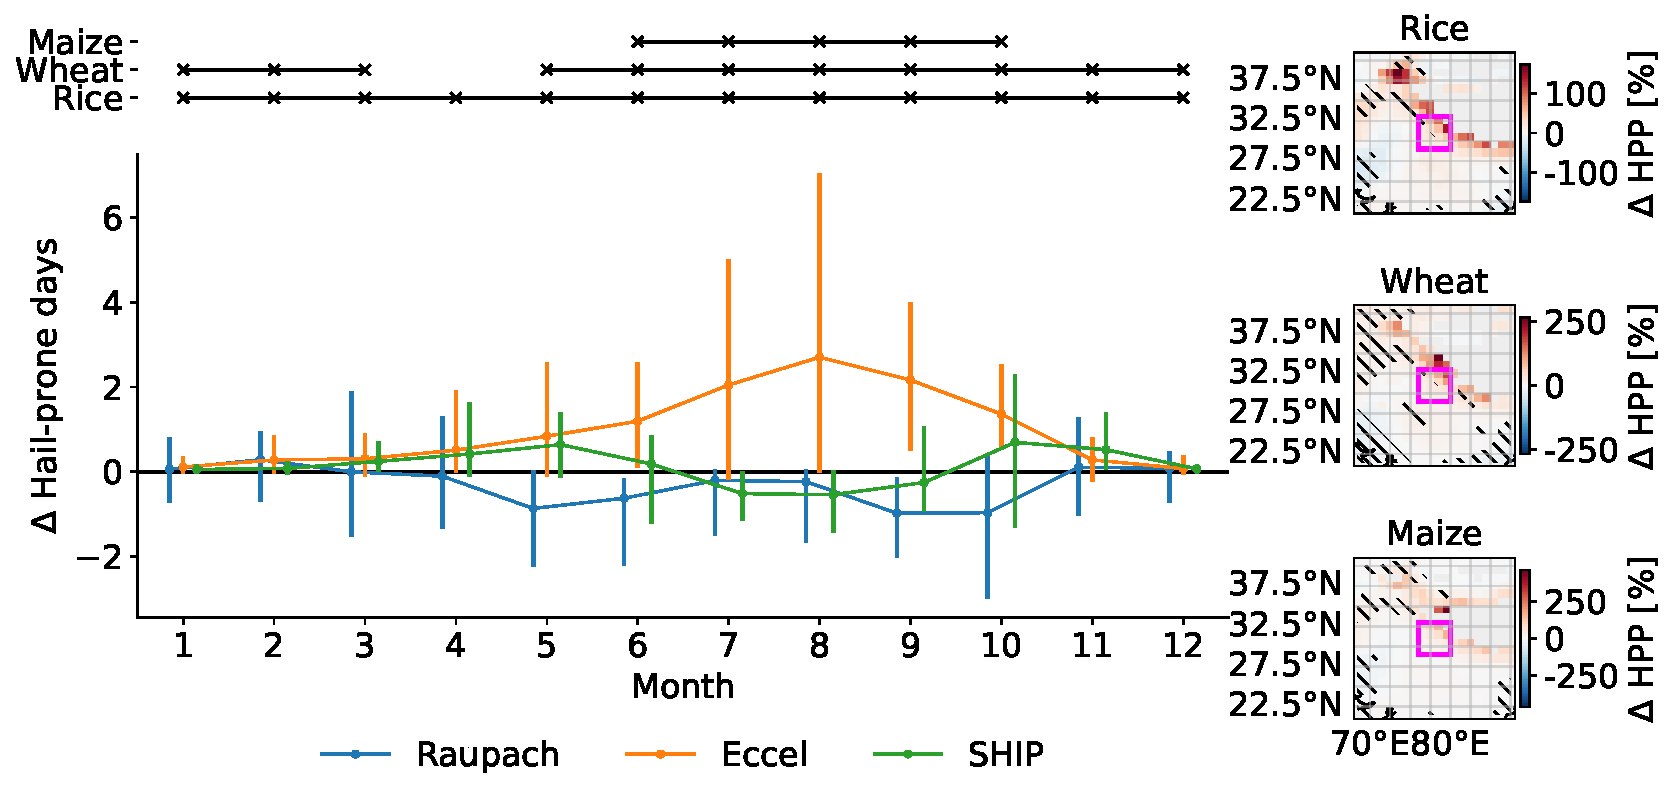
\includegraphics[width=\textwidth]{../../results/supplementary/crop_lines_india}
    \caption{As for Figure \ref{fig:crop_lines_af} but for India.}
    \label{fig:crop_lines_india}
\end{figure*}

\begin{figure*}[h]
    \centering
    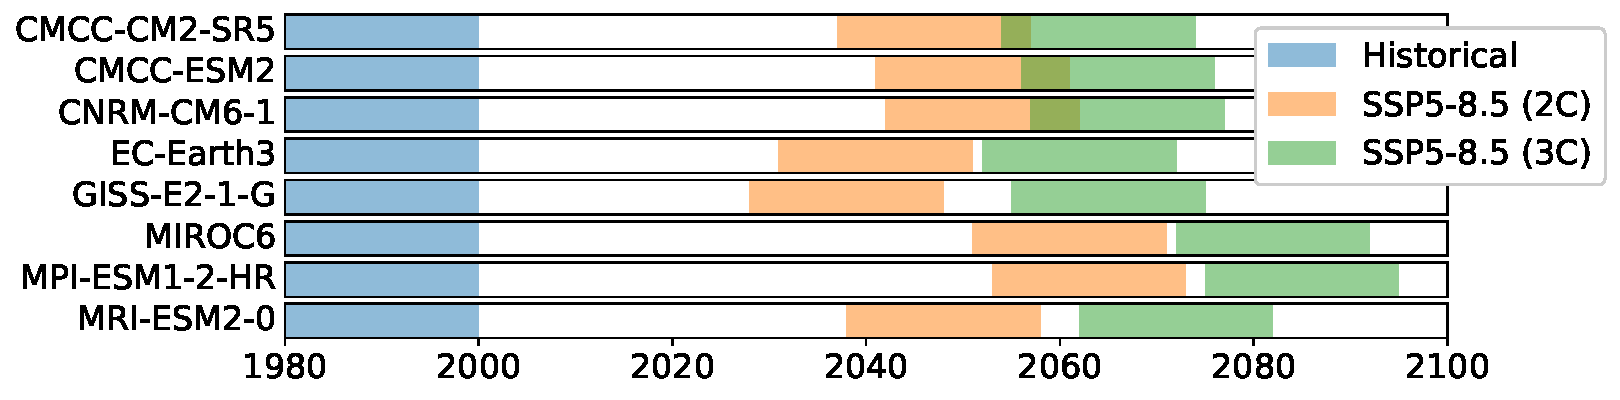
\includegraphics[width=\textwidth]{../../results/supplementary/run_years}
    \caption{\textbf{CMIP6 models and per-degree-framework date ranges.} The
    reference period from historical simulations is shown in blue, while periods
    with 2 and 3 \degr{} warming over the reference period, in SSP5-8.5
    simulations, are in orange and green respectively.}
    \label{fig:epochs}
\end{figure*}

\FloatBarrier
\newpage

\section{Proxy formulas}
\label{sec:proxy-formulas}

Three proxies were used in this work: Raupach, Eccel, and SHIP.

\subsection{Raupach proxy}
\label{sec:raupach_proxy}

The Raupach proxy is the modified proxy of Raupach et al., 2023
\cite{Raupach_MWR_2023}. This proxy was trained in Australia, a continent that
covers most types of hail environments, and the proxy was specifically designed
to adapt to latitudinal changes in hail environments \citep{Raupach_MWR_2023}.
Comparisons of proxy output with radar data showed reasonable co-fluctuation
\citep{Raupach_npjCAS_2023}. Here we slightly modified the original proxy to
make it more suitable for application in cold environments. The Raupach proxy
indicates hail-prone conditions when

\begin{eqnarray}
    \textrm{MLCAPE}_{100} \times {S_{06}}^\alpha & \geq & \beta, \label{eq:discrim} \\
    \textrm{LR} & < & -5.45 \textrm{ K km}^{-1} \label{eq:extra_conditions_1}, \\
    \textrm{LI}_{100} & < & 0.4 \textrm{ K} \label{eq:extra_conditions_2}, \\
    T_{500} & < & 265.46 \textrm{ K} \label{eq:extra_conditions_3},
\end{eqnarray}

where MLCAPE$_{100}$ (J kg$^{-1}$) is convective available potential energy
calculated using a well-mixed parcel over the lowest 100 hPa of the atmosphere,
$S_{06}$ (m s$^{-1}$) is 0-6 km bulk vertical wind shear, LR (K km$^{-1}$) is
the lapse rate between 700 hPa and 500 hPa, LI$_{100}$ (K) is the lifted index
\citep{Galway_BAMS_1956} defined using same parcel as that used by
MLCAPE$_{100}$, $T_{500}$ (K) is the temperature at 500 hPa, and $\alpha$ and
$\beta$ are parameters that vary with the melting level height such that

\begin{equation}
\alpha = 
    \begin{cases} 
        0.00127 \times \textrm{MLH} - 1.88272 & \textrm{ if }\quad\textrm{MLH} \geq 2000 \textrm{ m} \\
        0.00127 \times 2000 - 1.88272 & \textrm{ if }\quad\textrm{MLH} < 2000 \textrm{ m}\\
    \end{cases},
    \label{eq:newalpha}
\end{equation}

and 

\begin{equation}
\log_{10}(\beta) =
    \begin{cases}
    0.00204 \times \textrm{MLH} - 1.75631 & \textrm{ if }\quad\textrm{MLH} \geq 2000 \textrm{ m} \\
    0.00204 \times 2000 - 1.75631 & \textrm{ if }\quad\textrm{MLH} < 2000 \textrm{ m} \\
    \end{cases}.
    \label{eq:newbeta}
\end{equation}

\noindent where MLH (m) is melting level height, where wet-bulb temperature is
zero C, above sea level. The idea behind the parameters $\alpha$ and $\beta$ is
that there is a latitudinal dependence on the proportion of instability versus
shear in environments in which hailstorms occur in Australia
\citep{Raupach_MWR_2023}. Storms in the south, where shear is generally high and
melting level height is low, are more easily discriminated by MLCAPE$_{100}$
values, while storms in the tropics, where MLCAPE$_{100}$ and melting level
height are both generally high, are more easily discriminated by shear
\citep{Raupach_MWR_2023}. The proxy uses MLH to adjust the values of $\alpha$
and $\beta$ and therefore to adjust the discriminator between hail and no-hail
conditions in instability-shear space. 

\subsubsection{Modifications made to proxy}

In the original proxy of Raupach et al., 2023 \cite{Raupach_MWR_2023}, $\alpha$
and $\beta$ were set as follows:

\begin{eqnarray}
\alpha & = & 0.00127 \times \textrm{MLH} - 1.88272, \label{eq:alpha} \\
\log_{10}(\beta) & = & 0.00204 \times \textrm{MLH} - 1.75631. \label{eq:beta}
\end{eqnarray}

Figure \ref{fig:proxy_by_MLH} shows the original proxy \citep{Raupach_MWR_2023}
discriminator lines (set by Equations \ref{eq:discrim}, \ref{eq:alpha}, and
\ref{eq:beta}) for various values of melting level height (MLH). When the MLH is
below about 1500 m, the value of $\alpha$ becomes negative and the value of
$\beta$ becomes very small, and the proxy stops detecting high-CAPE, high-shear
conditions. So that the proxy is more reliable in colder regions where the
melting level height is below 1500 m, in this work we have modified the proxy
such that when the MLH is below 2000 m, the values of $\alpha$ and $\beta$ for
an MLH of 2000 m are used (Equations \ref{eq:newalpha} and \ref{eq:newbeta}).
This modification means the proxy is always able to detect high-CAPE, high-shear
conditions.

\begin{figure*}[!ht]
    \centering
    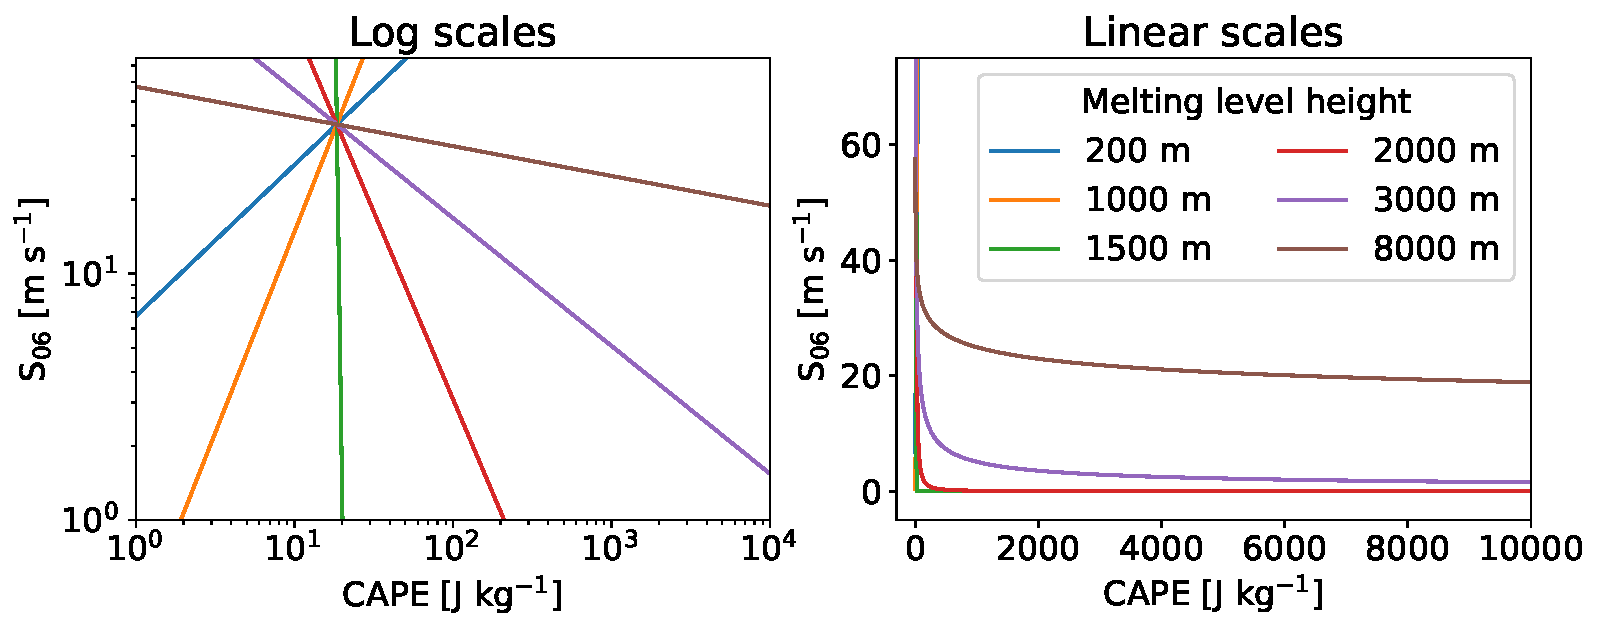
\includegraphics[width=\textwidth]{../../results/supplementary/proxy_by_MLH}
    \caption{\textbf{Original proxy for various values of melting level height
    (MLH).} CAPE stands for convective available potential energy. $S_{06}$ is
    0-6 km bulk vertical wind shear. The same discriminator lines are shown on
    logarithmic and linear scales.}
    \label{fig:proxy_by_MLH}
\end{figure*}

\subsubsection{Raupach proxy extra conditions}

Raupach et al., 2023 \cite{Raupach_MWR_2023} defined three ``extra conditions''
or thresholds (shown here as Equations \ref{eq:extra_conditions_1},
\ref{eq:extra_conditions_2}, and \ref{eq:extra_conditions_3}) designed to remove
false positives from hail-prone conditions produced by Equation
\ref{eq:discrim}. With and without the slight modification for MLH, our tests
showed these conditions are similarly effective in removing false positives from
the whole proxy training data set.  
It is notable that the projected changes in the updated Raupach proxy that we
report in this work are not driven primarily by the ``extra conditions'', as
shown by Supplementary Figure \ref{fig:Raupach_extra_conds}.

\begin{figure*}[h!]
    \centering
    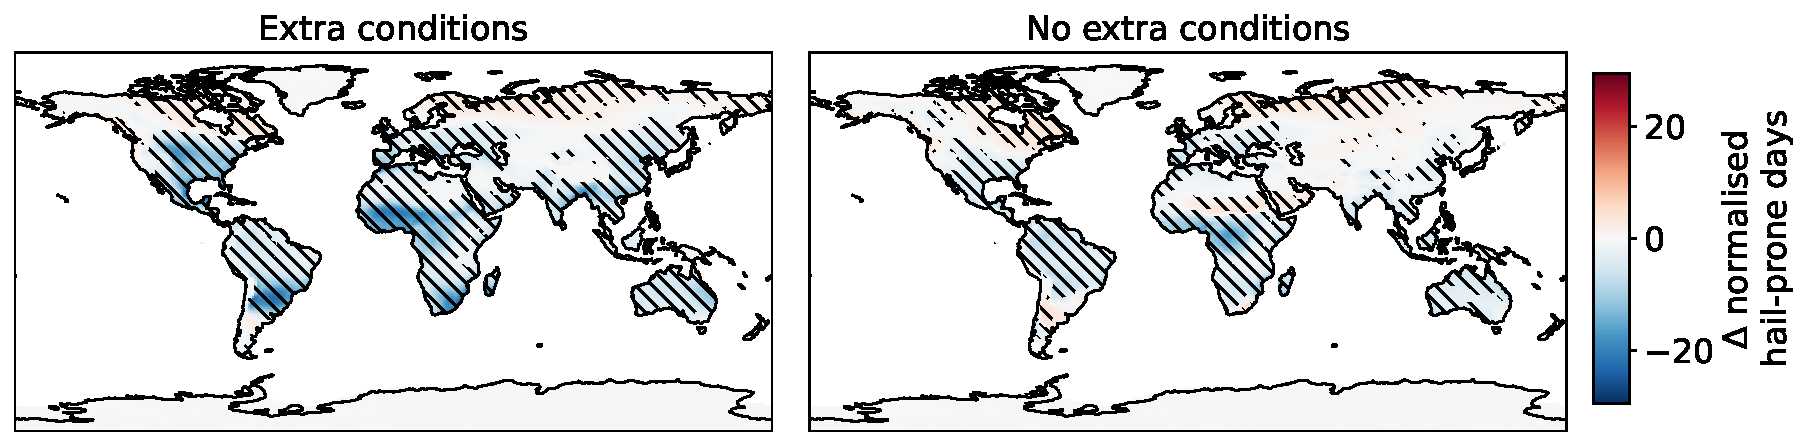
\includegraphics[width=\textwidth]{../../results/supplementary/Raupach_extra_conds_3C}
    \caption{\textbf{Effect of extra conditions on Raupach proxy for 3 \degr{}
    warming}. Changes shown are multimodel mean changes in annual hail-prone
    days. On left, the updated Raupach proxy with extra conditions applied; on
    right, changes in the updated Raupach proxy without extra conditions
    applied.}
    \label{fig:Raupach_extra_conds}
\end{figure*}

\subsubsection{Validation of modification}

To assess the impact of the changed calculation of $\alpha$ and $\beta$ we
tested on two datasets:

\begin{enumerate}
    \item On the original training dataset from Raupach et al., 2023
    \cite{Raupach_MWR_2023}: proxy performance metrics for the proxy with no
    extra conditions are similar between versions while the performance of the
    proxy with extra conditions is not affected by the change.
    \item On the climatology data used in Raupach et al., 2023
    \cite{Raupach_npjCAS_2023} covering storm-prone hours of the day from
    1979-2022 across all of Australia: the proxy changes affect the ocean areas
    in the south and southeast of the domain, with changes in mean annual
    hail-prone days of up to $\sim$2. However, over the whole map no location
    had more than
    0.67\%
    of its values affected and over land no location had more than
    0.35\%
    of its values affected. The climatology and trends calculated using either
    version of the proxy are very similar for Australia.
\end{enumerate}

\subsection{Eccel proxy}

The Eccel proxy, of Eccel et al., 2012 \cite{Eccel_IJC_2012}, defines an
environment as hail prone when 

\begin{eqnarray}
\textrm{MLCAPE}_{100} \times S_{06} > 10000,&\textrm{and} \\
\textrm{MLCIN}_{100} > -50,
\end{eqnarray}

where MLCIN$_{100}$ (J kg$^{-1}$) is convective inhibition for a well-mixed
parcel over the lowest 100 hPa of the atmosphere. 

\subsection{SHIP}

The SHIP proxy refers to the significant hail parameter
\citep[SHIP,][]{SPC_SHIP} which is defined by calculating an initial value,
SHIP$_i$, as

\begin{equation}
\textrm{SHIP}_i = \frac{\textrm{MUCAPE}_{250} \times \textrm{MR} \times \textrm{LR} \times -T_{500} \times S_{06}}{42000000},
\label{eq:SHIP}
\end{equation}

where MUCAPE$_{250}$ (J kg$^{-1}$) is the convective available potential energy
for the ``most unstable'' parcel, defined as the parcel with the largest
equivalent potential temperature over the lowest 250 hPa of the atmosphere, MR
(g kg$^{-1}$) is the mixing ratio for that parcel, and $T_{500}$ is the
temperature at 500 hPa in \degr{}. SHIP$_i$ is only defined when 

\begin{eqnarray}
7 \leq \textrm{S06} \leq 27 \textrm{ m s}^{-1}, & \textrm{and} \\
11 \leq \textrm{MR} \leq 13.6 \textrm{ g kg}^{-1}, &
\end{eqnarray}

and if $T_{500} > -5.5$ degrees C, then a value of $T_{500} = -5.5$ is used.
Once SHIP$_i$ has been calculated using Equation \ref{eq:SHIP} and these
constraints, the following modifications are made to get the final value of
SHIP:

\begin{eqnarray}
\textrm{SHIP} = \textrm{SHIP}_i \times \frac{\textrm{MUCAPE}_{250}}{1300}, & \textrm{if MUCAPE}_{250} < 1300 \textrm{ J kg}^{-1} \\ 
\textrm{SHIP} = \textrm{SHIP}_i \times \frac{\textrm{LR}}{5.8}, & \textrm{if LR} < 5.8 \textrm{ K km}^{-1} \\
\textrm{SHIP} = \textrm{SHIP}_i \times \frac{\textrm{FLH}}{2400}, & \textrm{if FLH} < 2400 \textrm{ m AGL},
\end{eqnarray}

where FLH is freezing-level height (height of dry-bulb zero degrees C) and AGL
stands for above ground level (note Raupach et al., 2023 \cite{Raupach_MWR_2023}
used FLH above sea level for Australia, but here we use FLH AGL as per both the
original SHIP definition and PH18). We considered an environment to be hail
prone when SHIP $> 0.1$, following Raupach et al., 2023 \cite{Raupach_MWR_2023}.

\subsection{Proxy normalisation}
\label{sec:proxy-normalisation}

The three proxies produced binary outputs, classifying each day as hail prone or
not hail prone. Annual hail-prone days were the sum of all hail-prone days per
year per location. To account for differences between the proxies and between
models, and to allow each proxy to have the same weight when calculating
multimodel, multi-proxy means, annual hail-prone days (AHPD) were normalised per
proxy and per model, such that

\begin{equation}
\textrm{AHPD}_{m,p,i,j,y} = \frac{\textrm{AHPD}_{m,p,i,j,y}}{\max\left([\textrm{AHPD}_{m,p,i,j,y}\;\forall\; i, j, y]\right)} \times 100,
\end{equation}

\noindent where $m$, $p$, $i$, $j$, $y$ are indices for model, proxy, longitude,
latitude, and year, respectively.

\FloatBarrier
\footnotesize

\bibliography{../main/library}

\end{document}
